% technical_manual_v2.tex — Furuno DRS4D-NXT Wire Protocol & System Technical Manual
% Author: J.C. Vaught
% Single self-contained LaTeX file with all figures inline via TikZ.

\documentclass[11pt,letterpaper]{article}

% ── Geometry ──────────────────────────────────────────────────────────────────
\usepackage[margin=1in]{geometry}

% ── Packages ──────────────────────────────────────────────────────────────────
\usepackage{tikz}
\usepackage{listings}
\usepackage{xcolor}
\usepackage{hyperref}
\usepackage{booktabs}
\usepackage{tabularx}
\usepackage{longtable}
\usepackage{fancyhdr}
\usepackage{amsmath,amssymb}
\usepackage{enumitem}
\usepackage{float}
\usepackage{caption}
\usepackage{graphicx}

% ── Brand Colors ──────────────────────────────────────────────────────────────
% Primary
\definecolor{Garnet}{HTML}{73000A}
\definecolor{Black}{HTML}{000000}
\definecolor{White}{HTML}{FFFFFF}
% Neutral
\definecolor{NinetyBlack}{HTML}{363636}
\definecolor{SeventyBlack}{HTML}{5C5C5C}
\definecolor{FiftyBlack}{HTML}{A2A2A2}
\definecolor{ThirtyBlack}{HTML}{C7C7C7}
\definecolor{TenBlack}{HTML}{ECECEC}
\definecolor{WarmGrey}{HTML}{676156}
\definecolor{Sandstorm}{HTML}{FFF2E3}
% Accent
\definecolor{Rose}{HTML}{CC2E40}
\definecolor{Atlantic}{HTML}{466A9F}
\definecolor{Congaree}{HTML}{1F414D}
\definecolor{Horseshoe}{HTML}{65780B}
\definecolor{Grass}{HTML}{CED318}
\definecolor{Honeycomb}{HTML}{A49137}

% ── Hyperref Setup ────────────────────────────────────────────────────────────
\hypersetup{
    colorlinks=true,
    linkcolor=Garnet,
    urlcolor=Atlantic,
    citecolor=Congaree,
    pdftitle={Furuno DRS4D-NXT --- Wire Protocol \& System Technical Manual},
    pdfauthor={J.C. Vaught},
}

% ── Section Heading Colors ────────────────────────────────────────────────────
\usepackage{titlesec}
\titleformat{\section}
    {\normalfont\Large\bfseries\color{Garnet}}{\thesection}{1em}{}
\titleformat{\subsection}
    {\normalfont\large\bfseries\color{NinetyBlack}}{\thesubsection}{1em}{}
\titleformat{\subsubsection}
    {\normalfont\normalsize\bfseries\color{SeventyBlack}}{\thesubsubsection}{1em}{}

% ── Header / Footer ──────────────────────────────────────────────────────────
\pagestyle{fancy}
\fancyhf{}
\fancyhead[L]{\small\color{SeventyBlack}Furuno DRS4D-NXT}
\fancyhead[R]{\small\color{SeventyBlack}Technical Manual}
\fancyfoot[C]{\small\color{FiftyBlack}\thepage}
\renewcommand{\headrulewidth}{0.4pt}
\renewcommand{\footrulewidth}{0pt}

% ── Code Listing Style ───────────────────────────────────────────────────────
\lstdefinestyle{code}{
    backgroundcolor=\color{TenBlack},
    basicstyle=\ttfamily\small,
    keywordstyle=\color{Garnet}\bfseries,
    stringstyle=\color{Atlantic},
    commentstyle=\color{FiftyBlack}\itshape,
    frame=single,
    framerule=0.4pt,
    rulecolor=\color{ThirtyBlack},
    framesep=6pt,
    xleftmargin=6pt,
    xrightmargin=6pt,
    breaklines=true,
    showstringspaces=false,
    tabsize=4,
}
\lstset{style=code}

% ── TikZ Libraries ───────────────────────────────────────────────────────────
\usetikzlibrary{arrows.meta, positioning, calc, shapes.geometric}

% ── Paragraph Spacing (no indent, half-line skip) ────────────────────────────
\setlength{\parindent}{0pt}
\setlength{\parskip}{0.5\baselineskip}

% ── No rounded corners globally ──────────────────────────────────────────────
\tikzset{every node/.append style={rounded corners=0pt}}

% ══════════════════════════════════════════════════════════════════════════════
\begin{document}

% ── Title Page ────────────────────────────────────────────────────────────────
\begin{titlepage}
    \centering
    \vspace*{2cm}

    {\Huge\bfseries\color{Garnet} Furuno DRS4D-NXT Radar}\\[0.5cm]
    {\LARGE\color{NinetyBlack} Wire Protocol \& System Technical Manual}\\[2cm]

    {\Large J.C. Vaught}\\[0.5cm]
    {\large\color{SeventyBlack} March 2026}\\[3cm]

    
\begin{tikzpicture}
        \fill[Garnet] (0,0) rectangle (10,0.15);
        \fill[Atlantic] (0,-0.3) rectangle (10,-0.15);
    \end{tikzpicture}

    \vfill
    {\normalsize\color{SeventyBlack}
    A complete technical reference for the Furuno DRS4D-NXT marine radar\\
    system, covering the wire protocol, echo data encoding, system\\
    architecture, web interface, and development guide.}
    \vspace{2cm}
\end{titlepage}

{\setlength{\parskip}{0pt}\tableofcontents}
\newpage


% ══════════════════════════════════════════════════════════════════════════════
%
%   PART I — OVERVIEW & USAGE
%
% ══════════════════════════════════════════════════════════════════════════════

\part{Overview \& Usage}
\label{part:usage}


% ──────────────────────────────────────────────────────────────────────────────
\section{Introduction}
\label{sec:introduction}

This document is the complete technical reference for the Furuno DRS4D-NXT marine radar system as interfaced through the \texttt{furuno-server} Rust application. It covers radar operation via a browser-based web interface, the internal software architecture, echo data encoding and decoding, and the full wire protocol. The intended audiences are new users learning to operate the system, contributors modifying the codebase, and developers building their own applications on top of the radar hardware.

\begin{figure}[H]
\centering
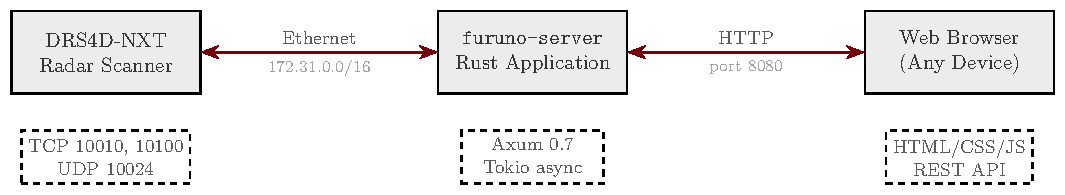
\includegraphics[width=0.95\textwidth]{figures/fig_system_overview.pdf}
\caption{System overview. The radar scanner communicates with the Rust server over a dedicated Ethernet link. The server exposes a web interface accessible from any browser on the network.}
\label{fig:system-overview}
\end{figure}

\subsection{Hardware Overview}
\label{subsec:hardware-overview}

The Furuno DRS4D-NXT is a solid-state Doppler marine radar operating in the X-band at 9.41~GHz. The scanner unit contains the antenna, transmitter, and receiver in a single sealed radome enclosure. It connects to a host processor via a standard Ethernet cable. The scanner is assigned a fixed IP address of \texttt{172.31.3.226} on a \texttt{172.31.0.0/16} subnet.

The radar transmits at up to 25~watts using solid-state amplification rather than a traditional magnetron, which eliminates warm-up time and provides consistent performance across the operating temperature range. The antenna rotates at either 24 or 48~RPM depending on the selected speed mode. Echo data is delivered as radial spokes, with 8192 unique azimuth positions per full rotation and up to 868 range bins per spoke. The system supports six pulse width settings (S1, S2, M1, M2, M3, L), 18 range scales from 1/16~NM to 48~NM, and built-in Doppler target discrimination.

\subsection{Software Components}
\label{subsec:software-components}

The system consists of three software components.

\textit{furuno-server} is a Rust binary that implements the complete Furuno wire protocol from scratch. It handles network discovery, authentication, control commands, echo data reception and decoding across four encoding types, PPI (Plan Position Indicator) rendering, and serves a web interface for browser-based operation. The application is built with Axum~0.7 for the HTTP server and Tokio for the async runtime. All radar communication---TCP control, UDP multicast echo reception, and subnet management---is handled natively without any Furuno proprietary libraries.

The \textit{web interface} is a set of static HTML, CSS, and JavaScript files served by the Rust application. It provides four pages: a controls dashboard for quick radar operation, a full-screen PPI display with history compositing, a detailed settings panel, and a system status view. The interface communicates with the server through a REST API and polls for updated radar images at 500\,ms intervals.

The \textit{documentation} consists of this technical manual and inline source code comments. The manual is maintained as a \LaTeX{} file with diagrams compiled as standalone PDFs from TikZ source files in the \texttt{figures/} directory.



% ──────────────────────────────────────────────────────────────────────────────
\newpage
\section{Quick Start \& Installation}
\label{sec:quickstart}

\subsection{Prerequisites}
\label{subsec:prerequisites}

The Rust toolchain is required to build the application. Install it via \texttt{rustup} if it is not already present.

\begin{lstlisting}[language=bash]
curl --proto '=https' --tlsv1.2 -sSf https://sh.rustup.rs | sh
source ~/.cargo/env
\end{lstlisting}

The application builds and runs on Linux (x86\_64 and aarch64), macOS, and Windows. No external C libraries or Furuno SDKs are required.

\subsection{Building}
\label{subsec:building}

From the repository root, build the release binary.

\begin{lstlisting}[language=bash]
cd furuno-server
cargo build --release
\end{lstlisting}

The compiled binary is located at \texttt{furuno-server/target/release/furuno-server}. A release build is recommended for deployment as it enables compiler optimizations that significantly improve echo decoding and PPI rendering throughput.

\subsection{First Run}
\label{subsec:first-run}

Start the web server with the \texttt{web} mode.

\begin{lstlisting}[language=bash]
cargo run --release -- web
\end{lstlisting}

The web interface is then available at \texttt{http://localhost:8080} in any browser. On startup, the application attempts to discover the radar automatically (see below). If the radar is not reachable, the web server starts anyway and serves a degraded interface. The \texttt{/reconnect} endpoint can be used to retry the connection later.

\subsection{Auto-Discovery}
\label{subsec:auto-discovery-quickstart}

The application resolves the radar and host IP addresses through a three-stage fallback process.

First, it checks for explicit command-line flags. If \texttt{-{}-radar-ip} is provided, that address is used directly. The \texttt{-{}-host-ip} flag is optional; if omitted, the application determines a suitable host address on the radar's subnet automatically.

\begin{lstlisting}[language=bash]
cargo run --release -- --radar-ip 172.31.3.226 web
\end{lstlisting}

Second, if no flags are provided, the application broadcasts UDP discovery beacons on port 10010 across all detected network interfaces and listens for 3 seconds. If the radar responds, both the radar and host addresses are extracted from the response.

Third, if discovery fails, the application falls back to the default addresses: \texttt{172.31.3.226} for the radar and \texttt{172.31.1.100} for the host. If the host does not already have an interface on the \texttt{172.31.0.0/16} subnet, a secondary IP alias is added to the physical Ethernet interface automatically. On Linux this uses \texttt{ip addr add}; on macOS, \texttt{ifconfig alias}.


% ──────────────────────────────────────────────────────────────────────────────
\newpage
\section{CLI Modes}
\label{sec:cli-modes-user}

\subsection{General Syntax}
\label{subsec:cli-syntax}

The application accepts optional IP flags followed by a mode name and mode-specific arguments.

\begin{lstlisting}[language=bash]
furuno-server [--radar-ip IP] [--host-ip IP] <mode> [args...]
\end{lstlisting}

The two user-facing modes are \texttt{web} and \texttt{discover}. Additional developer-oriented modes (\texttt{handshake}, \texttt{tx-on}, \texttt{tx-off}, \texttt{echo}, \texttt{full}, \texttt{render-live}, \texttt{dump-raw}, \texttt{test-commands}, \texttt{validate}) are documented in \S\ref{sec:cli-modes-dev}. If no mode is given, the application defaults to \texttt{handshake}.

\subsection{Web Server Mode}
\label{subsec:cli-web}

The \texttt{web} mode starts the HTTP server and is the primary way to operate the radar.

\begin{lstlisting}[language=bash]
furuno-server web [port] [webdir]
\end{lstlisting}

The optional \texttt{port} argument sets the listening port (default 8080). The optional \texttt{webdir} argument specifies the path to the static web files (default \texttt{../web} relative to the binary). On startup, the server attempts to authenticate with the radar and initialize the control channel. If the radar is unreachable, the server starts anyway with degraded functionality---the PPI display shows a blank image and setting changes are queued until a connection is established via the \texttt{/reconnect} endpoint.

\subsection{Discover Mode}
\label{subsec:cli-discover}

The \texttt{discover} mode broadcasts UDP beacons on port 10010 across all network interfaces and prints any radar responses it receives.

\begin{lstlisting}[language=bash]
furuno-server discover
\end{lstlisting}

This is useful for determining the radar's IP address on an unfamiliar network or verifying that the radar is powered on and reachable. The mode runs until a response is received or the timeout expires.


% ──────────────────────────────────────────────────────────────────────────────
\newpage
\section{Web Interface}
\label{sec:web-interface}

\subsection{Starting the Server}
\label{subsec:starting-server}

The web server starts when the application is launched in \texttt{web} mode (see \S\ref{subsec:cli-web}). By default it listens on port 8080 and serves static files from the \texttt{../web} directory relative to the binary. Both values can be overridden with positional arguments. The server starts even if the radar is not reachable, allowing the interface to load and wait for a connection. The \texttt{/reconnect} API endpoint triggers a fresh authentication and initialization attempt without restarting the server.

\subsection{Page Tour}
\label{subsec:page-tour}

The web interface consists of four HTML pages, all sharing a common header with navigation links, a consistent CSS stylesheet, and a single shared JavaScript file (\texttt{script.js}).

\subsubsection{Controls (index.html)}
\label{subsubsec:page-controls}

The controls page is the default landing page and provides the most commonly used radar operations. It is divided into two panels. The left panel displays a radar preview image (refreshed every 2 seconds) with a link to the full-screen radar view. The right panel contains quick controls for TX power (on/off), CSV recording (start/stop), range selection (17 scales from 0.0625 to 36~NM), pulse width (S1 through L), manual gain (0--100), and RezBoost level (off/low/medium/high). Each control has an apply button and a refresh button that queries the radar's current state.

Below the quick controls is a pattern loader panel. Users can load a pattern file (\texttt{.txt} or \texttt{.csv}), set a repeat count ($-1$ for infinite looping), assign an optional label, and add the pattern to a queue. The queue is displayed as an ordered list, and patterns execute sequentially when the RUN button is pressed. A STOP button halts execution mid-pattern, and RESET clears the queue.

\begin{figure}[H]
\centering
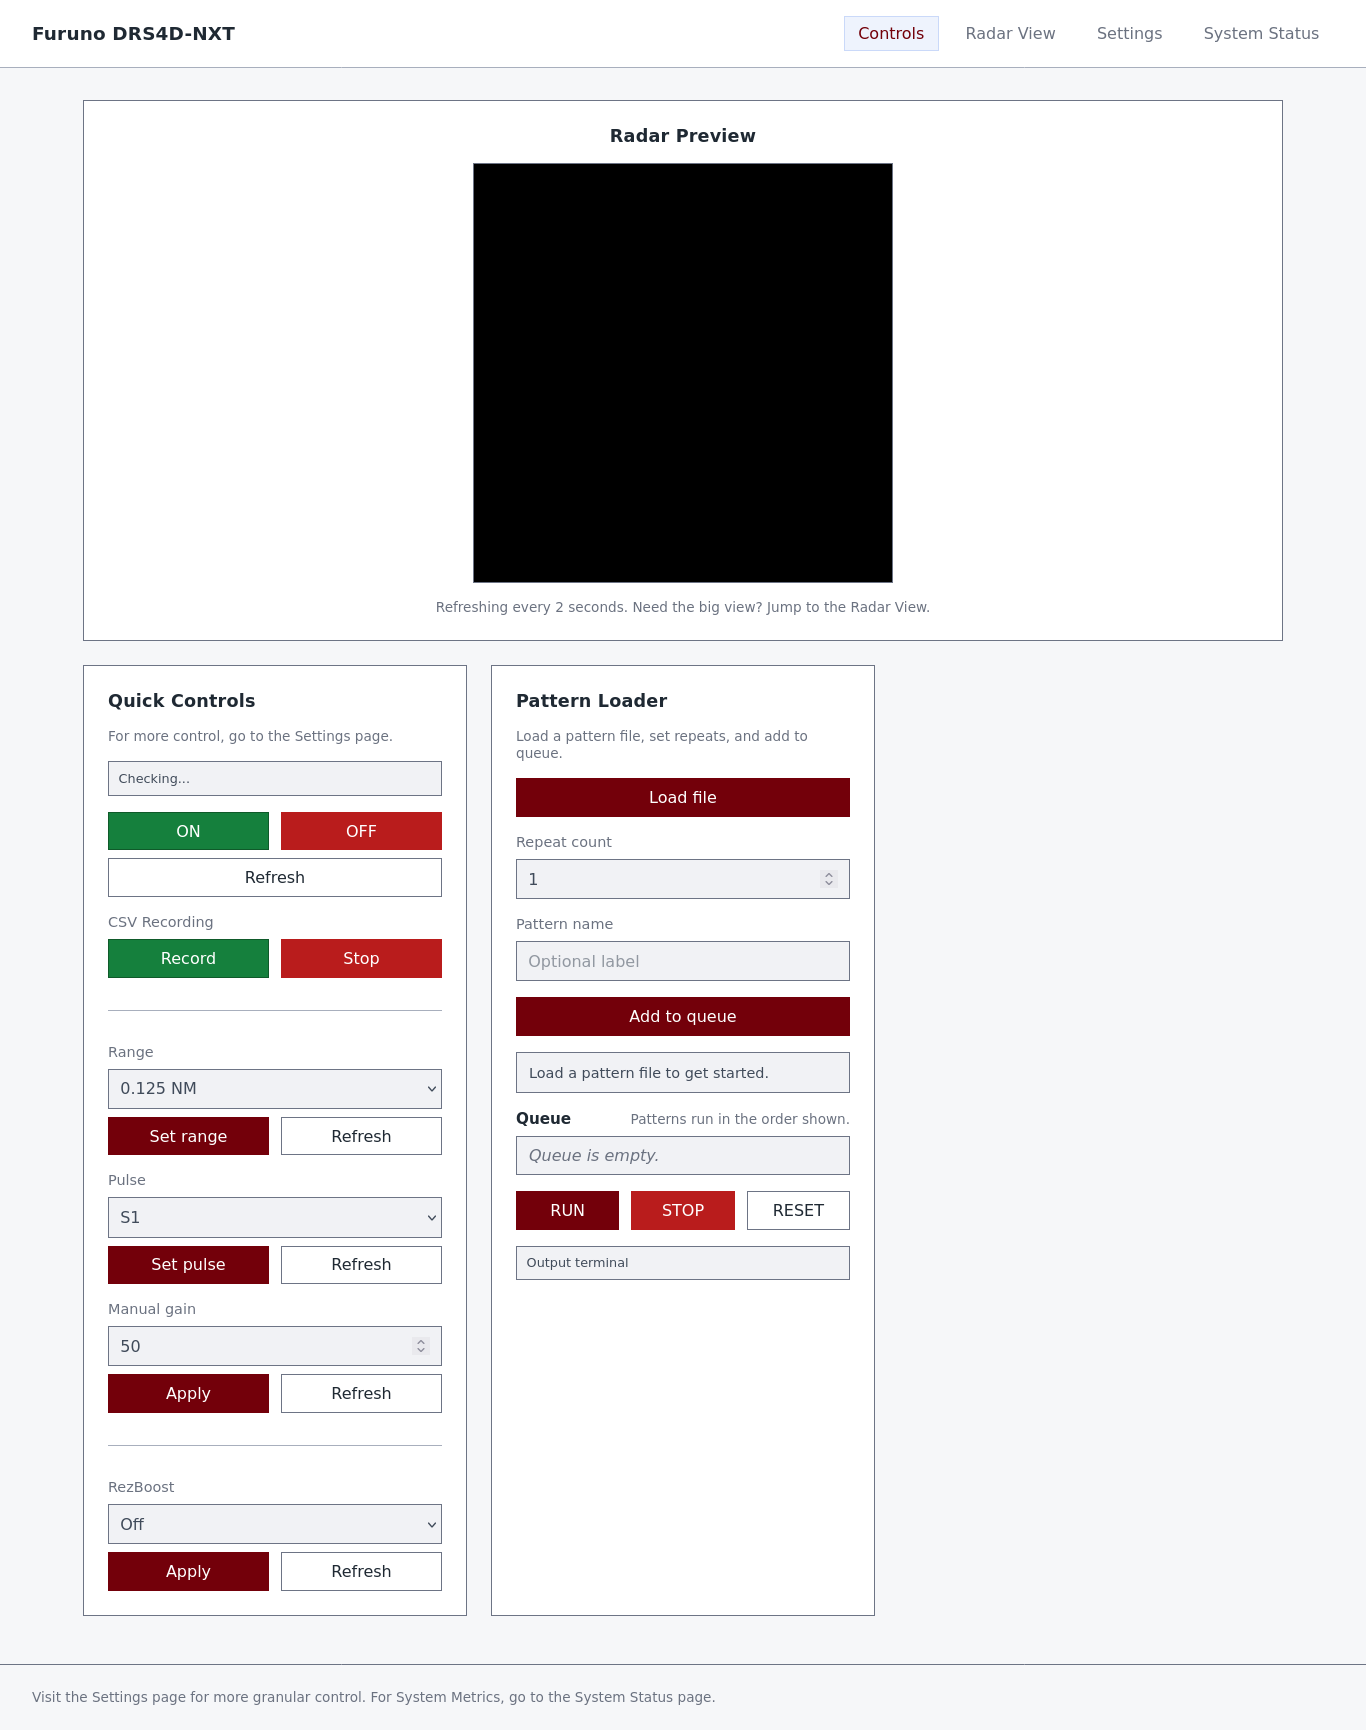
\includegraphics[width=0.85\textwidth]{figures/screenshot_controls.png}
\caption{Controls page (\texttt{index.html}). The radar preview is shown at top, with quick controls and the pattern loader below.}
\label{fig:page-controls}
\end{figure}

\subsubsection{Radar View (radar.html)}
\label{subsubsec:page-radar}

The radar view page provides a full-screen PPI display. The primary display element is an HTML5 canvas (1024$\times$1024 pixels) that composites multiple frames of radar data to show target history. Below the canvas are controls for track length (1--50 frames), current frame color, and track history color, with a reset button to restore defaults. An \texttt{<img>} element behind the canvas serves as a fallback if canvas rendering is unavailable. The canvas is refreshed every 500\,ms by fetching the latest PPI image from the \texttt{/newest\_png} endpoint.

% To add this screenshot: save as figures/screenshot_radar.png
\IfFileExists{figures/screenshot_radar.png}{
\begin{figure}[H]
\centering
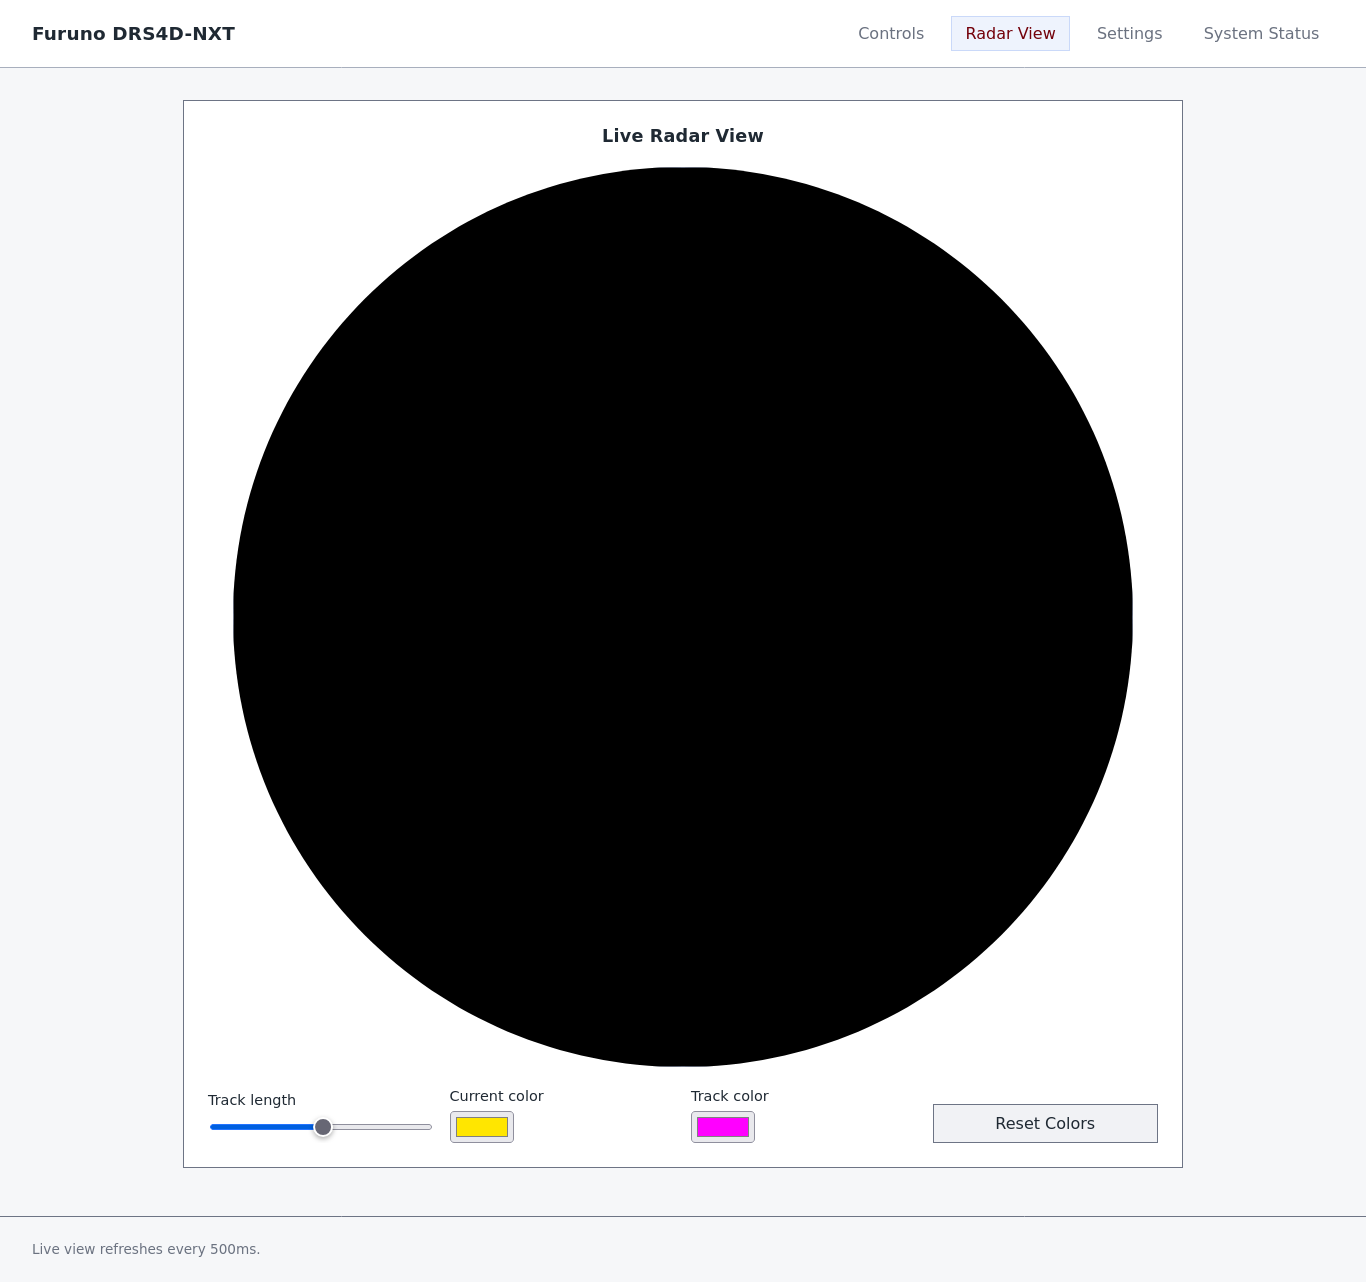
\includegraphics[width=0.85\textwidth]{figures/screenshot_radar.png}
\caption{Radar view page (\texttt{radar.html}). The PPI display with history compositing and track color controls.}
\label{fig:page-radar}
\end{figure}
}{}

\subsubsection{Settings (settings.html)}
\label{subsubsec:page-settings}

The settings page provides granular control over all radar parameters. It is organized into panels grouped by function.

The \textit{connection panel} shows the current connection status and provides reconnect and refresh buttons. A small radar preview image is displayed alongside.

The \textit{power control panel} provides TX on/off buttons and a refresh button to query the current transmitter state.

The \textit{range and pulse panel} allows independent or combined adjustment of range and pulse width, with the same options available on the controls page.

The \textit{gain panel} supports both manual and automatic gain modes. In manual mode, the user sets a value from 0 to 100. In auto mode, a bias offset (0--100) adjusts how aggressively the automatic gain control responds.

The \textit{STC panel} exposes three sensitivity time control zones---near, mid, and far---each with an independent numeric input.

The \textit{signal processing panel} groups main bang suppression (0--255), interference rejection (on/off), bird mode (off/low/medium/high), and Doppler target analysis (off, internal heading, external heading).

The \textit{clutter panel} provides sea clutter (A/C SEA) and rain clutter (A/C RAIN) controls, each with manual and automatic modes. Manual mode sets a fixed rejection level; auto mode adjusts a bias for the radar's internal adaptive filter.

The \textit{antenna speed panel} controls rotation speed (auto/low/high) and a high-RPM override toggle.

The \textit{RezBoost and display panel} sets the resolution enhancement level and display parameters including sweep line count and interpolation mode.

The \textit{pattern loader} on this page has the same functionality as the one on the controls page, with the addition of a manual text input option for entering pattern steps directly.

\IfFileExists{figures/screenshot_settings_top.png}{
\begin{figure}[H]
\centering
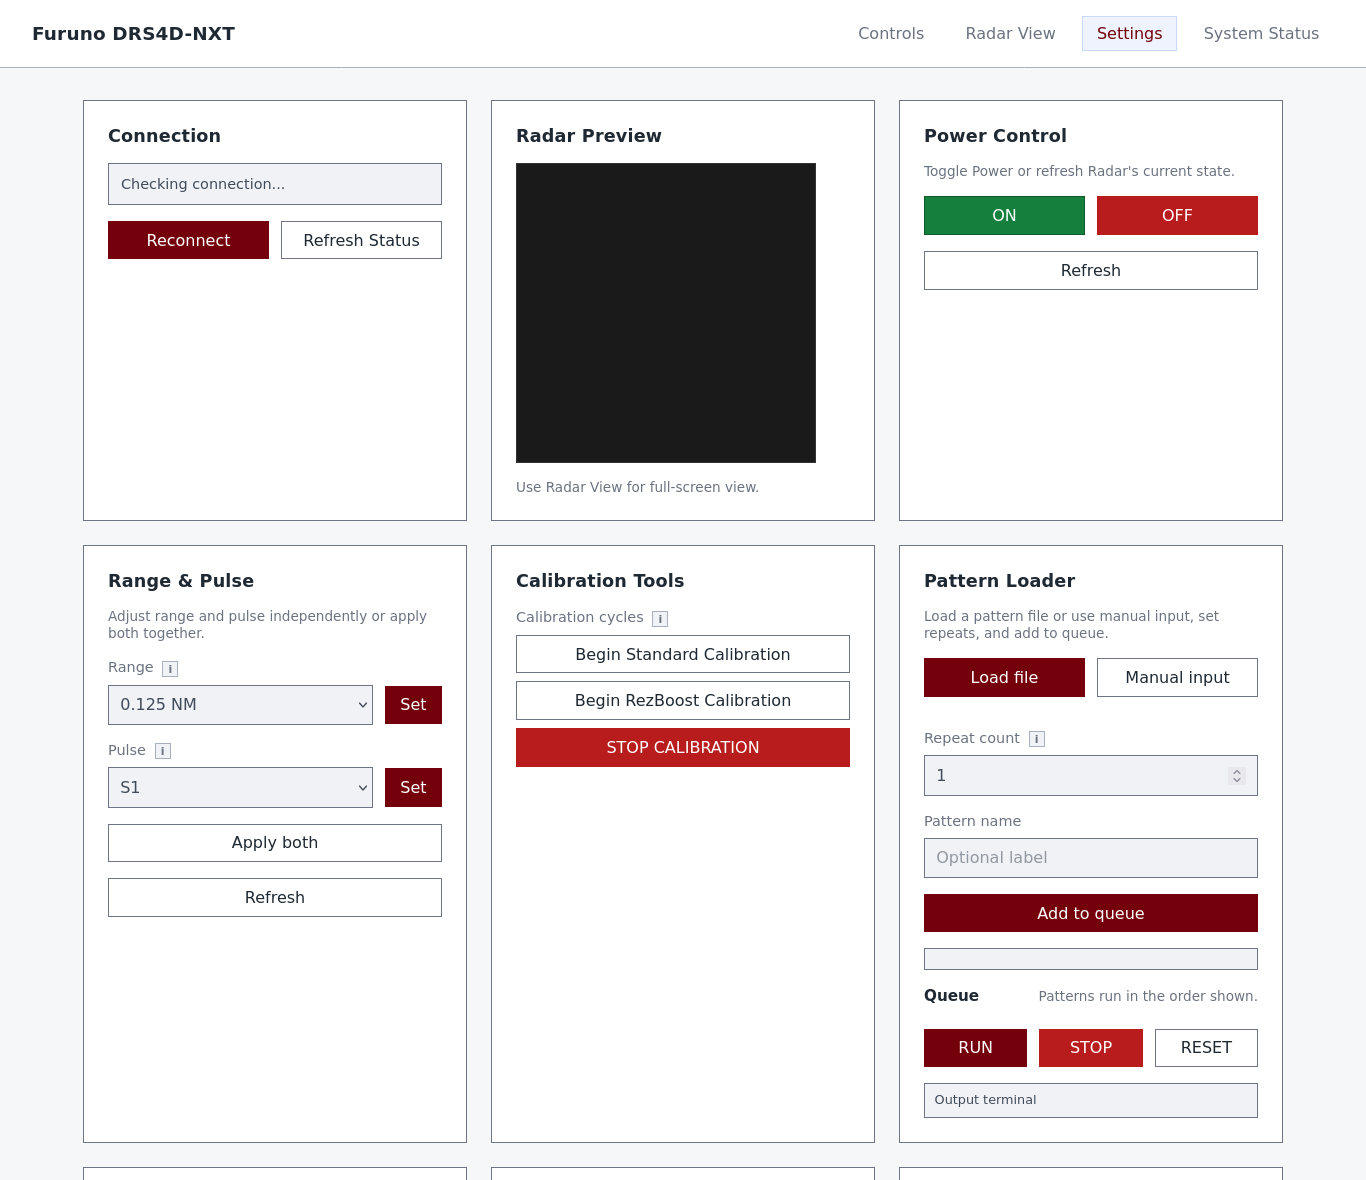
\includegraphics[width=0.85\textwidth]{figures/screenshot_settings_top.png}
\caption{Settings page (\texttt{settings.html}), upper half. Connection, radar preview, power control, range/pulse, calibration tools, and pattern loader panels.}
\label{fig:page-settings-top}
\end{figure}
}{}

\IfFileExists{figures/screenshot_settings_bottom.png}{
\begin{figure}[H]
\centering
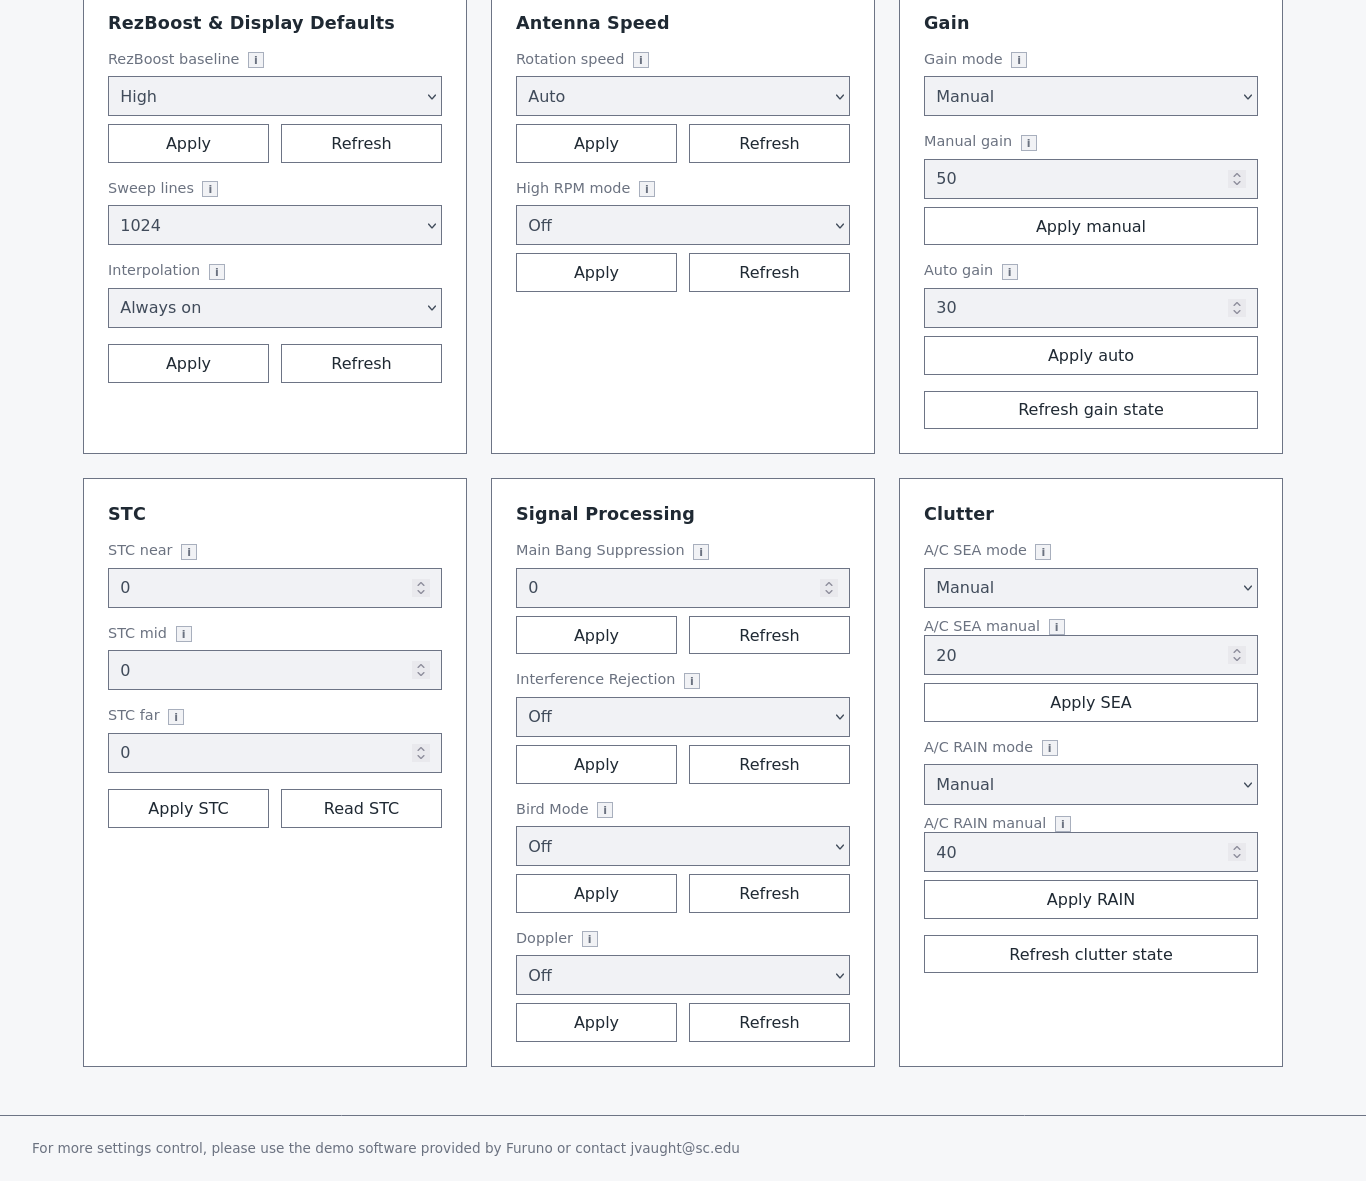
\includegraphics[width=0.85\textwidth]{figures/screenshot_settings_bottom.png}
\caption{Settings page (\texttt{settings.html}), lower half. RezBoost, antenna speed, gain, STC, signal processing, and clutter panels.}
\label{fig:page-settings-bottom}
\end{figure}
}{}

\subsubsection{System Status (status.html)}
\label{subsubsec:page-status}

The system status page displays live telemetry from both the radar and the host system, updated every 500\,ms.

The \textit{radar connection} panel shows connection status, radar IP, host IP, TX state, and firmware version. The \textit{session} panel shows server uptime, total rotations received, recording state, the current recording directory, and pattern queue status. The \textit{active settings} panel displays a read-only summary of all current radar parameters: range, pulse, gain, RezBoost, antenna speed, Doppler, interference rejection, bird mode, main bang suppression, STC values, and clutter settings.

The \textit{host resources} panels display CPU load (overall and per-core), memory usage, storage usage, network throughput, and CPU temperature. Each metric includes a progress bar and numeric label.

% To add this screenshot: save as figures/screenshot_status.png
\IfFileExists{figures/screenshot_status.png}{
\begin{figure}[H]
\centering
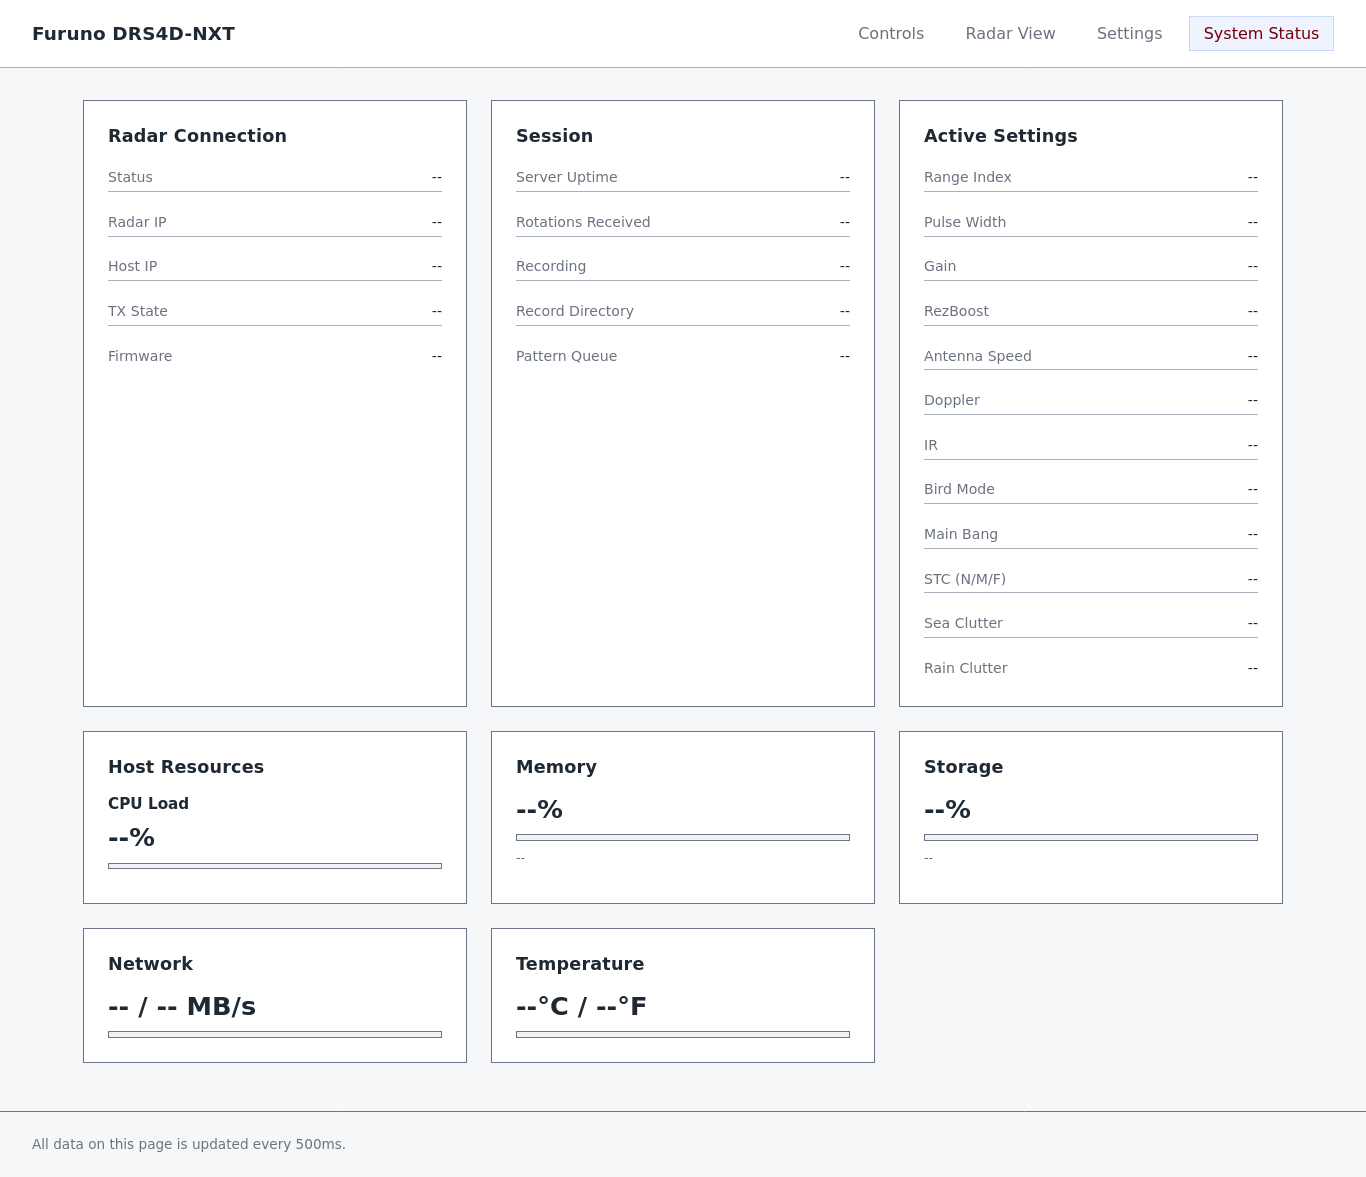
\includegraphics[width=0.85\textwidth]{figures/screenshot_status.png}
\caption{System status page (\texttt{status.html}). Live telemetry from the radar and host system.}
\label{fig:page-status}
\end{figure}
}{}

\subsection{PPI Display}
\label{subsec:ppi-display}

The PPI (Plan Position Indicator) display renders radar echo data as a top-down circular image with the radar at the center. The server renders each complete antenna rotation into a 640$\times$640 pixel PNG image using the warm-tinted color mapping described in \S\ref{subsec:color-mapping}. The browser fetches the latest image via the \texttt{/newest\_png} endpoint.

On the radar view page, the JavaScript composites multiple frames onto an HTML5 canvas to show target motion history. The \textit{track length} slider controls how many previous frames are retained (1--50). The \textit{current color} picker tints the most recent frame, and the \textit{track color} picker tints older frames. Older frames are drawn with decreasing opacity to produce a fading trail effect. This compositing runs entirely in the browser; the server delivers only single-frame PNG images.


% ──────────────────────────────────────────────────────────────────────────────
\newpage
\section{Recording \& Data Formats}
\label{sec:recording}

\subsection{Starting and Stopping Recording}
\label{subsec:recording-toggle}

Recording is toggled through the web interface or by calling the \texttt{/toggle\_recording} API endpoint with a \texttt{state} parameter of \texttt{start} or \texttt{stop}. When recording starts, the server creates a new timestamped directory under \texttt{recordings/} with \texttt{csv/} and \texttt{png/} subdirectories. If a directory with the same timestamp already exists, a numeric suffix is appended (e.g., \texttt{\_01}, \texttt{\_02}). Each complete antenna rotation produces one CSV file and one PNG file, written automatically by the echo listener thread. When recording is stopped, a \texttt{settings.json} snapshot is written to the recording directory.

\subsection{Output Directory Structure}
\label{subsec:recording-directory}

Each recording session produces the following directory structure.

\begin{lstlisting}
recordings/<timestamp>/
  csv/rotation_<ts>.csv
  png/rotation_<ts>.png
  settings.json
\end{lstlisting}

The top-level directory is named with a compact timestamp (e.g., \texttt{20260307\_143022}). For pattern-based recordings, the sanitized pattern label is appended (e.g., \texttt{20260307\_143022\_sweep1}). The \texttt{csv/} and \texttt{png/} subdirectories are created on demand when the first rotation is written.

\subsection{CSV Format}
\label{subsec:csv-format}

Each CSV file represents one complete antenna rotation. The file begins with a metadata header of \texttt{\#}-prefixed comment lines that capture all radar settings at the time of recording.

\begin{lstlisting}
# range_index,4
# gain_auto,false
# gain_value,50
# pulse_width,0
# sea_clutter,0
# rain_clutter,0
# rezboost,0
# interference_rejection,false
# bird_mode,0
# doppler,0
# antenna_speed,0
# main_bang,0
# near_stc,0
# middle_stc,0
# far_stc,0
Status	Scale	Range	Gain	Angle	EchoValues
0	4	4	19	0	12,14,8,...
0	4	4	19	1	10,11,9,...
\end{lstlisting}

After the header, the column line and data rows are tab-separated. Each row represents one spoke and contains a status field (always 0), the range scale index, the range index, the gain percentage (mapped from the 0--255 wire range to 0--100), the azimuth angle in ticks (0--8191), and the echo bin values as a comma-separated list of integers.

\subsection{Settings Snapshot}
\label{subsec:settings-snapshot}

When a recording session ends, the server writes a \texttt{settings.json} file to the recording directory. The snapshot format depends on how the recording was initiated.

For manual recordings, the snapshot contains the mode (\texttt{"manual"}), the recording directory path, the full \texttt{CurrentSettings} object, and a \texttt{history} array of \texttt{SettingChange} entries. Each history entry records a timestamp, the setting name, and the new value, capturing every parameter change made during the recording session.

For pattern-based recordings, the snapshot additionally includes the \texttt{PatternInfo} object describing the pattern that was executing, including all pattern steps with their parameter values and repeat counts.


% ──────────────────────────────────────────────────────────────────────────────
\newpage
\section{Pattern System}
\label{sec:pattern-system}

\subsection{What Patterns Do}
\label{subsec:pattern-overview}

Patterns automate sequences of radar parameter changes. A pattern consists of one or more \textit{steps}, each specifying a set of radar settings and a \textit{repeat count} that determines how many full antenna rotations that step is held before advancing to the next. When recording is active during pattern execution, each rotation produces a CSV and PNG file, allowing systematic data collection across parameter combinations.

\begin{figure}[H]
\centering
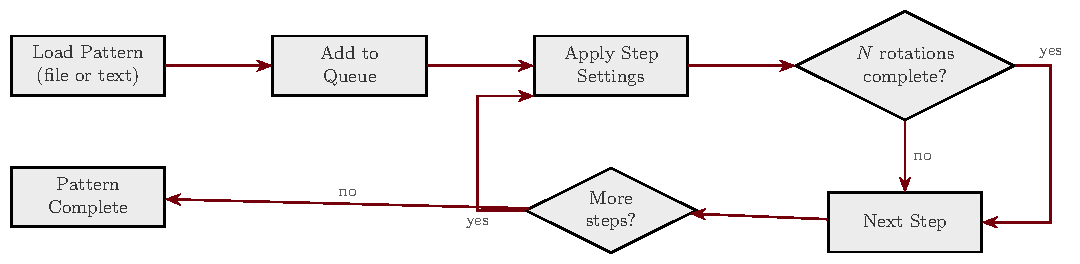
\includegraphics[width=0.95\textwidth]{figures/fig_pattern_flow.pdf}
\caption{Pattern execution flow. Each step is applied to the radar and held for the specified number of antenna rotations before advancing.}
\label{fig:pattern-flow}
\end{figure}

\subsection{Simple Pattern Format (7-Field)}
\label{subsec:pattern-simple}

The simple format uses seven comma-separated fields per step. All fields are required and all values are set explicitly.

\begin{lstlisting}
range, gain, pulse, rezboost, speed, interp, repeat
\end{lstlisting}

For example, the step \texttt{4,50,0,3,2,1,5} sets range index 4 (1~NM), gain 50, pulse S1, RezBoost high, auto antenna speed, interpolation on, and holds for 5 rotations. Multiple steps are separated by semicolons.

\begin{lstlisting}
4,50,0,3,2,1,5; 8,50,2,3,2,1,5; 11,50,4,3,2,1,5
\end{lstlisting}

\subsection{Advanced Pattern Format (13-Field)}
\label{subsec:pattern-advanced}

The advanced format extends the simple format with six additional fields for fine-grained signal processing control.

\begin{lstlisting}
range, gain, pulse, rezboost, speed, interp,
    sea_clutter, rain_clutter, main_bang,
    interference_rejection, bird_mode, doppler, repeat
\end{lstlisting}

Any of the 12 parameter fields (all except \texttt{repeat}) can be set to \texttt{NaN} to leave that setting unchanged from its current value. This is particularly useful when only a subset of parameters needs to vary across steps. For example, the step \texttt{4,NaN,0,NaN,NaN,NaN,NaN,NaN,NaN,NaN,NaN,NaN,3} changes only the range to index 4 and the pulse to S1, leaving all other settings at their current values and holding for 3 rotations.

\subsection{Pattern Queue}
\label{subsec:pattern-queue}

Multiple patterns can be loaded into a queue and executed sequentially. Each queue entry has its own pattern data, repeat count, and optional label. The repeat count controls how many times the entire pattern is cycled ($-1$ for infinite looping). Patterns execute in the order they were added.

During queue execution, each pattern item creates its own recording session with a separate timestamped directory (tagged with the sanitized pattern label if one was provided). The queue can be stopped at any time using the STOP button, which halts execution between steps. A RESET button clears the entire queue.

\subsection{Loading Patterns}
\label{subsec:pattern-loading}

Patterns can be loaded in two ways. The first is file upload: clicking the ``Load file'' button opens a file picker that accepts \texttt{.txt} or \texttt{.csv} files. The file contents are parsed as semicolon-separated steps. The second is manual input: on the settings page, clicking ``Manual input'' reveals a text area where steps can be typed or pasted directly.

After loading, the user sets a repeat count and an optional label, then clicks ``Add to queue'' to append the pattern to the queue list. Multiple patterns can be queued before pressing RUN.

\subsection{NaN Override Behavior}
\label{subsec:pattern-nan}

When a pattern step uses \texttt{NaN} for a field, that setting remains \textit{unlocked} during execution. This means the user can manually change that parameter through the web UI while the pattern runs, and the change takes effect immediately. Conversely, parameters with explicit values in the current step are \textit{locked}---manual changes to locked parameters are rejected with an error message indicating that the setting is controlled by the active pattern.

This mechanism allows hybrid operation where some parameters are swept by the pattern while others are adjusted interactively. For example, a pattern that sweeps range and pulse but sets all clutter fields to \texttt{NaN} lets the operator tune clutter rejection in real time while the automated sweep runs.


% ══════════════════════════════════════════════════════════════════════════════
%
%   PART II — SOFTWARE INTERNALS
%
% ══════════════════════════════════════════════════════════════════════════════

\newpage
\part{Software Internals}
\label{part:internals}


% ──────────────────────────────────────────────────────────────────────────────
\section{System Architecture Overview}
\label{sec:architecture}

This section provides a high-level map of the codebase. Each subsystem is introduced briefly here and covered in depth in subsequent sections.

\subsection{Module Summary}
\label{subsec:module-summary}

The Rust server is organized into the following source modules, all compiled as a single binary via \texttt{main.rs}.

\begin{table}[H]
\centering
\begin{tabularx}{\textwidth}{l l X}
\toprule
\textbf{File} & \textbf{Role} & \textbf{Details} \\
\midrule
\texttt{main.rs} & Entry point & CLI argument parsing, IP resolution, mode dispatch \\
\texttt{protocol.rs} & Wire protocol & Packet encoding/decoding, command builders, echo decompression \\
\texttt{connection.rs} & State machine & TCP auth, control channel, keepalives, response parsing (\S\ref{sec:connection-state-machine}) \\
\texttt{web.rs} & Web server & Axum HTTP handlers, echo listener thread, recording, pattern engine (\S\ref{sec:web-server}--\S\ref{sec:pattern-engine}) \\
\texttt{echo.rs} & Echo helpers & Rotation collection, CSV export, echo header parsing \\
\texttt{render.rs} & PPI renderer & Polar-to-Cartesian projection, color mapping, PNG encoding (\S\ref{sec:ppi-rendering}) \\
\texttt{modes.rs} & CLI modes & Standalone operations: handshake, TX control, dump, render-live (\S\ref{sec:cli-modes-dev}) \\
\texttt{testing.rs} & Test harness & A/B command verification, 6-phase validation suite (\S\ref{sec:testing}) \\
\texttt{tests.rs} & Unit tests & \texttt{\#[cfg(test)]} integration tests requiring live radar \\
\bottomrule
\end{tabularx}
\caption{Source module summary.}
\label{tab:modules}
\end{table}

\subsection{System-Level Block Diagram}
\label{subsec:system-diagram}

The following diagram shows the physical and network boundaries of the system. The radar hardware communicates with the Rust server over a dedicated Ethernet link, and the server exposes an HTTP interface to the browser.

\begin{figure}[H]
\centering
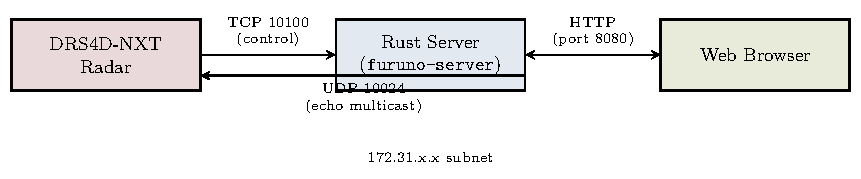
\includegraphics[width=0.85\textwidth]{figures/fig_system_blocks.pdf}
\caption{System-level block diagram showing radar hardware, Rust server, and browser.}
\label{fig:system-blocks}
\end{figure}

\subsection{Module-Level Diagram}
\label{subsec:module-diagram}

\begin{figure}[H]
\centering
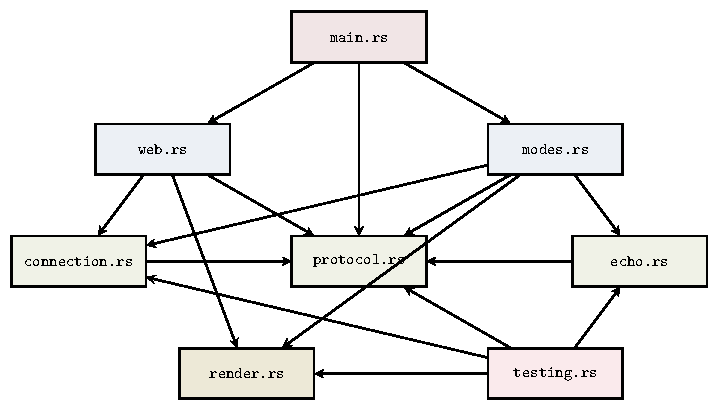
\includegraphics[width=0.7\textwidth]{figures/fig_module_deps.pdf}
\caption{Module dependency diagram. Arrows point from dependent module to dependency.}
\label{fig:module-deps}
\end{figure}

\subsection{Data Flow Diagram}
\label{subsec:dataflow-diagram}

\begin{figure}[H]
\centering
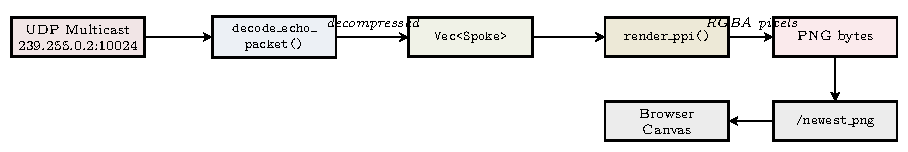
\includegraphics[width=0.95\textwidth]{figures/fig_dataflow.pdf}
\caption{Echo data flow from UDP multicast to browser canvas.}
\label{fig:dataflow}
\end{figure}

\subsection{Concurrency Model}
\label{subsec:concurrency}

The server uses a hybrid concurrency model combining Tokio async tasks with a dedicated OS thread.

The \textbf{Tokio async runtime} handles all HTTP request processing. Each Axum handler runs as an async task on the Tokio thread pool. Blocking radar operations (sending commands, waiting for acknowledgments) are wrapped in \texttt{tokio::task::spawn\_blocking()} to avoid blocking the async executor.

A single \textbf{dedicated \texttt{std::thread}} runs the echo listener loop. This thread receives UDP multicast packets, decodes spokes, renders the PPI image, and optionally writes CSV/PNG files during recording. It runs independently of the HTTP handlers and communicates with them through shared state.

\textbf{Synchronization primitives} in the shared \texttt{AppState} struct coordinate access between the async handlers and the echo thread. \texttt{Mutex<RadarConnection>} provides exclusive access to the TCP control channel, ensuring only one thread sends commands at a time. \texttt{RwLock<Vec<u8>{}>} protects the latest PNG image, allowing the echo thread to write and multiple HTTP handlers to read concurrently. Several \texttt{AtomicBool} flags (\texttt{tx\_active}, \texttt{recording}, \texttt{pattern\_stop}) provide lock-free coordination for frequently checked boolean state.


% ──────────────────────────────────────────────────────────────────────────────
\newpage
\section{PPI Rendering}
\label{sec:ppi-rendering}

The PPI (Plan Position Indicator) renderer in \texttt{render.rs} converts a vector of decoded \texttt{Spoke} structs into a $640 \times 640$ pixel RGBA image. This is the most commonly modified subsystem when changing visual appearance, image resolution, or overlay elements.

\subsection{Coordinate Transformation}
\label{subsec:coordinate-transform}

Each spoke has an \texttt{angle\_ticks} field representing a compass bearing (0 = north, increasing clockwise) in the range 0--8191 (8192 ticks per full rotation). The renderer converts this to a standard math angle (0 = east, increasing counter-clockwise) using the formula:
\begin{align}
\theta_{\text{rad}} &= \frac{\texttt{angle\_ticks}}{8192} \times 2\pi \\
\theta_{\text{math}} &= \frac{\pi}{2} - \theta_{\text{rad}}
\end{align}

For each spoke, the renderer walks outward from the image center along the radial line defined by $\theta_{\text{math}}$, one pixel step at a time. At each step at radius $r$, the corresponding range bin index is calculated by linear interpolation:
\begin{equation}
\texttt{bin} = \left\lfloor \frac{r}{r_{\max}} \times N_{\text{bins}} \right\rfloor
\end{equation}
where $r_{\max} = 318$ pixels (center minus 2-pixel margin) and $N_{\text{bins}} = 868$ (the standard number of range bins per spoke). The pixel coordinates are:
\begin{align}
p_x &= \texttt{center} + r \cdot \cos(\theta_{\text{math}}) \\
p_y &= \texttt{center} - r \cdot \sin(\theta_{\text{math}})
\end{align}

\subsection{Color Mapping}
\label{subsec:color-mapping}

Echo amplitudes arrive as 6-bit values (0--63) after the \texttt{wire >> 2} display conversion. The renderer scales these to 8-bit intensity and applies a warm-tinted color mapping:
\begin{align}
\texttt{intensity} &= \min\!\left(\frac{\texttt{amplitude} \times 255}{63},\; 255\right) \\[4pt]
R &= \texttt{intensity} \\
G &= \left\lfloor \texttt{intensity} \times \frac{180}{255} \right\rfloor \approx 0.706 \times \texttt{intensity} \\
B &= \left\lfloor \texttt{intensity} \times \frac{20}{255} \right\rfloor \approx 0.078 \times \texttt{intensity}
\end{align}

This produces a warm amber/orange color for strong returns, fading to dark red/brown for weak returns. Zero-amplitude bins are left as the black background (RGBA 0,0,0,255).

\subsection{Overlay Elements}
\label{subsec:overlays}

After all spokes are drawn, the renderer adds two overlay elements in dark gray (RGB 54, 54, 54).

\textbf{Crosshairs} are drawn as a horizontal and vertical line passing through the image center, spanning the full image width and height.

\textbf{Range rings} are drawn as four equally-spaced circles at radii $r_{\max}/4$, $r_{\max}/2$, $3r_{\max}/4$, and $r_{\max}$. Each ring is rasterized by stepping around its circumference with angular resolution proportional to its perimeter.

\subsection{PNG Encoding}
\label{subsec:png-encoding}

Two functions handle PNG output, both using the \texttt{png} crate.

\texttt{encode\_png\_bytes(pixels, width, height)} encodes the RGBA pixel buffer into an in-memory \texttt{Vec<u8>} containing the complete PNG file. This is used by the echo listener thread to update the \texttt{latest\_png} shared state without touching the filesystem.

\texttt{write\_png(path, pixels, width, height)} writes the PNG directly to a file via a buffered writer. This is used during recording (per-rotation PNG saves) and by CLI modes that produce output files.

Both functions encode as RGBA color type with 8-bit depth.

\subsection{How to Modify}
\label{subsec:ppi-how-to-modify}

\textbf{Image size.} Change the \texttt{PPI\_SIZE} constant (currently 640). All geometry is computed relative to this value, so no other changes are needed. Larger sizes produce smoother radial lines at the cost of increased memory and PNG encoding time.

\textbf{Color palette.} Modify the three lines in \texttt{render\_ppi()} that assign to \texttt{pixels[idx]}, \texttt{pixels[idx+1]}, and \texttt{pixels[idx+2]}. For a green phosphor look, use $R = 0$, $G = \texttt{intensity}$, $B = 0$. For a blue-white scheme, use $R = \texttt{intensity}/2$, $G = \texttt{intensity}/2$, $B = \texttt{intensity}$.

\textbf{New overlays.} Add drawing code after the range ring loop in \texttt{render\_ppi()}. The pixel buffer is a flat \texttt{Vec<u8>} in row-major RGBA order. The index for pixel $(x, y)$ is $(y \times \texttt{size} + x) \times 4$, with offsets +0 for R, +1 for G, +2 for B, +3 for A.


% ──────────────────────────────────────────────────────────────────────────────
\newpage
\section{Web Server}
\label{sec:web-server}

The web server in \texttt{web.rs} is the primary interface for operating the radar. It serves both the static HTML/CSS/JS files and a REST API for controlling radar parameters and retrieving data.

\subsection{Framework}
\label{subsec:web-framework}

The server is built on \textbf{Axum 0.7}, a Rust web framework that runs on the \textbf{Tokio} async runtime. The \texttt{start\_server()} function is annotated with \texttt{\#[tokio::main]} to create the async runtime. All HTTP handlers are async functions, with blocking radar I/O operations wrapped in \texttt{tokio::task::spawn\_blocking()} to prevent stalling the event loop.

Key dependencies: \texttt{axum} for routing and extraction, \texttt{tower-http} for static file serving, \texttt{serde} for query parameter deserialization, and \texttt{serde\_json} for JSON responses.

\subsection{Shared State}
\label{subsec:appstate}

All server state lives in a single \texttt{AppState} struct, wrapped in \texttt{Arc} and passed to every handler via Axum's \texttt{State} extractor. The key fields and their synchronization primitives are listed below.

\begin{table}[H]
\centering
\begin{tabularx}{\textwidth}{l l X}
\toprule
\textbf{Field} & \textbf{Type} & \textbf{Purpose} \\
\midrule
\texttt{conn} & \texttt{Mutex<RadarConnection>} & Exclusive access to the TCP control channel \\
\texttt{latest\_png} & \texttt{RwLock<Vec<u8>{}>} & Most recent PPI image (PNG-encoded bytes) \\
\texttt{tx\_active} & \texttt{AtomicBool} & Whether the transmitter is currently on \\
\texttt{connected} & \texttt{AtomicBool} & Whether the radar connection is established \\
\texttt{recording} & \texttt{AtomicBool} & Whether CSV/PNG recording is active \\
\texttt{record\_dir} & \texttt{RwLock<String>} & Current recording output directory path \\
\texttt{rotation\_count} & \texttt{AtomicU64} & Total antenna rotations since server start \\
\texttt{pattern\_stop} & \texttt{AtomicBool} & Signal to abort a running pattern \\
\texttt{pattern\_running} & \texttt{AtomicBool} & Whether a pattern is currently executing \\
\texttt{pattern\_status} & \texttt{RwLock<String>} & Human-readable pattern execution status \\
\texttt{settings} & \texttt{RwLock<CurrentSettings>} & Current radar configuration for CSV metadata \\
\texttt{setting\_history} & \texttt{RwLock<Vec<SettingChange>{}>} & Change log for recording snapshots \\
\texttt{host\_ip} & \texttt{Ipv4Addr} & Host IP (used by echo socket) \\
\texttt{start\_time} & \texttt{Instant} & Server start time (for uptime calculation) \\
\bottomrule
\end{tabularx}
\caption{\texttt{AppState} fields and synchronization.}
\label{tab:appstate}
\end{table}

\subsection{Route Registration}
\label{subsec:route-registration}

Routes are registered in \texttt{start\_server()} using Axum's \texttt{Router} builder. Each route maps a URL path to a handler function. All routes use the \texttt{GET} method except \texttt{/run\_pattern\_queue} which uses \texttt{POST} (for large JSON payloads). The router ends with a \texttt{fallback\_service(ServeDir::new(web\_dir))} that serves static files from the \texttt{web/} directory for any path that does not match a registered route.

Several legacy aliases exist for backward compatibility: \texttt{/begin\_calibration} and \texttt{/run\_ramp\_pattern} both map to the same handler as \texttt{/run\_pattern}.

\subsection{Handler Pattern}
\label{subsec:handler-pattern}

All handlers follow a consistent pattern:

\begin{lstlisting}[basicstyle=\small\ttfamily]
async fn handle_set_range(
    State(state): State<Arc<AppState>>,
    Query(params): Query<RangeParams>,
) -> String {
    // Build command from params
    // Send via spawn_blocking + send_cmd()
    // Update settings, return status string
}
\end{lstlisting}

The \texttt{State} extractor provides access to the shared \texttt{AppState}. The \texttt{Query} extractor deserializes URL query parameters into a typed struct. Handlers that modify radar settings also update the \texttt{CurrentSettings} in shared state and log a \texttt{SettingChange} entry for recording metadata.

The helper function \texttt{send\_cmd()} wraps the blocking radar I/O pattern: it takes a command string and expected acknowledgment prefix, calls \texttt{send\_and\_read\_ack()} inside \texttt{spawn\_blocking()}, and returns a status message.

\subsection{Echo Listener Thread}
\label{subsec:echo-listener}

A dedicated \texttt{std::thread} (spawned at server startup) runs the \texttt{echo\_listener()} function. This thread joins the UDP multicast group 239.255.0.2:10024 and continuously receives echo packets.

The listener maintains a running buffer of spokes for the current rotation. When it detects a rotation wrap (azimuth drops by more than 1000 ticks from the previous spoke), it renders the accumulated spokes into a PPI image via \texttt{render\_ppi()}, encodes it to PNG via \texttt{encode\_png\_bytes()}, and stores the result in \texttt{latest\_png}. If recording is active, it also writes a CSV and PNG file to the recording directory.

The listener sends keepalive packets every 5 seconds (via \texttt{try\_lock()} on the connection mutex) and drains pending control channel data. When TX is not active, it sleeps in 100\,ms intervals to avoid busy-waiting.

\subsection{Static File Serving}
\label{subsec:static-files}

The \texttt{tower\_http::services::ServeDir} middleware serves the \texttt{web/} directory as a fallback for any path not matched by an explicit route. By default, the web directory is \texttt{../web} relative to the binary location. This can be overridden with the second positional argument to the \texttt{web} CLI mode.

The static files include \texttt{index.html}, \texttt{radar.html}, \texttt{settings.html}, \texttt{status.html}, \texttt{styles.css}, and \texttt{script.js}. The JavaScript in \texttt{script.js} handles page-specific logic including polling \texttt{/newest\_png} every 500\,ms, sending API requests, and managing pattern queue state.

\subsection{How to Add a New Endpoint}
\label{subsec:add-endpoint}

To add a new endpoint, follow these steps.

\begin{enumerate}[leftmargin=2em]
\item \textbf{Define a parameter struct.} Create a \texttt{\#[derive(Deserialize)]} struct with fields matching the expected query parameters. Use \texttt{\#[serde(rename = "camelCase")]} for JavaScript-friendly names.

\item \textbf{Write the handler.} Create an async function taking \texttt{State(state): State<Arc<AppState>{}>} and \texttt{Query(params): Query<YourParams>}. Use \texttt{send\_cmd()} for radar commands, or access shared state directly for read-only queries.

\item \textbf{Register the route.} Add a \texttt{.route("/your\_endpoint", get(handle\_your\_endpoint))} line in the router chain in \texttt{start\_server()}.
\end{enumerate}


% ──────────────────────────────────────────────────────────────────────────────
\newpage
\section{REST API Reference}
\label{sec:rest-api}

All endpoints are verified against the source code in \texttt{web.rs}. Unless otherwise noted, all endpoints accept \texttt{GET} requests with URL query parameters and return plain text responses.

\subsection{Power and Connection}
\label{subsec:api-power}

\begin{longtable}{l p{10cm}}
\toprule
\textbf{Endpoint} & \textbf{Description} \\
\midrule
\texttt{/toggle\_echo?mode=on|off} & Turn the transmitter on or off. Accepts optional \texttt{radarNo} parameter (ignored). \\
\texttt{/reconnect} & Drop the current connection and re-establish auth, control channel, and init. Resets TX state to off. \\
\bottomrule
\end{longtable}

\subsection{Settings}
\label{subsec:api-settings}

All settings endpoints accept \texttt{GET} requests with query parameters. During pattern execution, manual changes to pattern-controlled settings are rejected unless the pattern step uses \texttt{NaN} for that field.

\begin{longtable}{l p{9cm}}
\toprule
\textbf{Endpoint} & \textbf{Parameters} \\
\midrule
\texttt{/set\_range} & \texttt{rangeIndex} (0--17) \\
\texttt{/set\_pulse\_width} & \texttt{pulse} (0--5: S1/S2/M1/M2/M3/L), optional \texttt{rangeIndex} \\
\texttt{/set\_gain} & \texttt{status} (0=manual, 1=auto), \texttt{manualValue} (0--255), \texttt{autoValue} \\
\texttt{/set\_acsea} & \texttt{status}, \texttt{manual} (0--255), \texttt{auto}, \texttt{mode} (0=Advanced, 1=Coastal) \\
\texttt{/set\_acrain} & \texttt{status}, \texttt{manual} (0--255), \texttt{auto}, \texttt{ftcMode} (0/1/2), \texttt{rainMode} (0/1/2) \\
\texttt{/set\_bearing\_resolution} & \texttt{mode} (0--3: Off/Low/Med/High) \\
\texttt{/set\_antenna\_revolution} & \texttt{rollSpeed} (0=Lo, 1=Hi, 2=Auto), \texttt{hiRpm} (0/1) \\
\texttt{/set\_near\_stc} & \texttt{value} (0--4) \\
\texttt{/set\_middle\_stc} & \texttt{value} (0--3) \\
\texttt{/set\_far\_stc} & \texttt{value} (0--2) \\
\texttt{/set\_main\_bang} & \texttt{value} (0--255) \\
\texttt{/set\_interference\_rejection} & \texttt{enabled} (0=off, 1=on) \\
\texttt{/set\_bird\_mode} & \texttt{level} (0--3: Off/Low/Med/High) \\
\texttt{/set\_doppler} & \texttt{mode} (0=Off, 1=Internal heading, 2=External heading) \\
\bottomrule
\end{longtable}

\subsection{State Queries}
\label{subsec:api-state}

\begin{longtable}{l p{9cm}}
\toprule
\textbf{Endpoint} & \textbf{Description} \\
\midrule
\texttt{/get\_current} & Query a specific setting from the radar. \texttt{command} parameter selects the setting: \texttt{TX}, \texttt{RANGE}, \texttt{PULSE}, \texttt{GAIN}, \texttt{CLUTTER}, \texttt{ANTENNA}, \texttt{STC}, \texttt{MAINBANG}, \texttt{IR}, \texttt{BIRDMODE}, \texttt{DOPPLER}, \texttt{SWEEP}. Optional \texttt{format=json} for JSON response (STC only). \\
\texttt{/get\_system\_info} & Returns JSON with full system state: connection status, TX state, firmware, IPs, recording state, rotation count, uptime, pattern status, current settings, memory and storage usage. \\
\texttt{/system\_metrics} & Returns JSON with host system metrics: per-core CPU usage, load average, memory usage, storage usage, network throughput, and CPU temperature. \\
\bottomrule
\end{longtable}

\subsection{Echo Image}
\label{subsec:api-echo-image}

\texttt{GET /newest\_png} returns the most recent PPI image as \texttt{image/png} with \texttt{Cache-Control: no-cache}. If no echo data has been received yet, returns a 1$\times$1 black pixel PNG as a placeholder. The browser JavaScript polls this endpoint every 500\,ms to update the radar display.

\subsection{Recording}
\label{subsec:api-recording}

\texttt{GET /toggle\_recording?mode=start|stop} starts or stops recording. When started, creates a timestamped directory under \texttt{recordings/} with \texttt{csv/} and \texttt{png/} subdirectories, and writes a \texttt{settings.json} snapshot. Each completed rotation during recording produces a CSV and PNG file in the respective subdirectories.

\subsection{Pattern Execution}
\label{subsec:api-patterns}

\begin{longtable}{l l p{7cm}}
\toprule
\textbf{Endpoint} & \textbf{Method} & \textbf{Description} \\
\midrule
\texttt{/run\_pattern} & GET & Execute a single pattern. \texttt{steps} (semicolon-separated), \texttt{repeat} count, optional \texttt{label}. \\
\texttt{/run\_pattern\_queue} & POST & Execute a queue of patterns. JSON body with base64-encoded \texttt{payload} containing pattern items. \\
\texttt{/stop\_pattern} & GET & Set the \texttt{pattern\_stop} flag to abort the current pattern. \\
\texttt{/pattern\_status} & GET & Returns a JSON object with current pattern execution status, active step info, and queue progress. \\
\bottomrule
\end{longtable}

Legacy aliases \texttt{/begin\_calibration} and \texttt{/run\_ramp\_pattern} both map to the same handler as \texttt{/run\_pattern}.

\subsection{Stub Endpoints}
\label{subsec:api-stubs}

\texttt{/set\_sweep\_total} and \texttt{/set\_interpolation} are registered routes that return \texttt{"OK"} without performing any action. These exist for compatibility with the web interface JavaScript, which sends requests to these endpoints. The sweep total is fixed at the PPI resolution (640$\times$640) and interpolation is handled client-side.


% ──────────────────────────────────────────────────────────────────────────────
\newpage
\section{Recording System Internals}
\label{sec:recording-internals}

This section describes how the recording system works internally. For user-facing recording instructions, see \S\ref{sec:recording}.

\subsection{Echo Listener Integration}
\label{subsec:recording-echo-listener}

Recording is triggered by the echo listener thread, not by the HTTP handlers. When the \texttt{recording} flag is set to \texttt{true} and the echo listener detects a rotation wrap (azimuth drops by more than 1000 ticks), it writes the completed rotation's data to disk before clearing the spoke buffer.

The echo listener checks \texttt{state.recording.load(Ordering::Relaxed)} on every rotation boundary. If recording is active and \texttt{record\_dir} is non-empty, it writes both a CSV file and a PNG file for that rotation. This tight coupling with the echo thread ensures every rotation is captured without gaps.

\subsection{Directory Creation}
\label{subsec:recording-directory-creation}

When recording starts, a timestamped directory is created under \texttt{recordings/}. The directory name encodes the date and time (e.g., \texttt{recordings/20260307\_143022/}). Two subdirectories are created inside: \texttt{csv/} for spoke data files and \texttt{png/} for rendered PPI images. The path is stored in \texttt{state.record\_dir} so the echo listener thread can find it.

If the recording was triggered by a pattern queue, the directory is created per-pattern-item, with each item getting its own timestamped directory and \texttt{settings.json} snapshot.

\subsection{CSV Writing}
\label{subsec:recording-csv-writing}

The \texttt{write\_echo\_csv()} function in \texttt{web.rs} writes a single rotation's data to a CSV file. Each file begins with \texttt{\#}-prefixed metadata lines containing the current radar settings at the time of capture. These metadata lines record every field from \texttt{CurrentSettings}: range index and label, gain mode and value, pulse width, sea clutter, rain clutter, RezBoost level, interference rejection state, bird mode, Doppler mode, antenna speed, main bang suppression, near/middle/far STC values.

After the metadata header, a column header line defines the fields: \texttt{spoke\_index}, \texttt{angle\_ticks}, \texttt{angle\_deg}, \texttt{heading\_ticks}, \texttt{num\_bins}, followed by \texttt{bin\_0} through \texttt{bin\_867}. Each subsequent line contains one spoke's data. Spokes with fewer than the maximum number of bins are zero-padded.

\subsection{Settings Snapshots}
\label{subsec:recording-snapshots}

A \texttt{settings.json} file is written to the recording directory when recording starts. The schema depends on how recording was initiated.

\textbf{Manual recording} produces a \texttt{ManualRecordingSettingsSnapshot} containing the mode (\texttt{"manual"}), the recording directory path, the full \texttt{CurrentSettings} object, and the setting change history accumulated since the server started.

\textbf{Pattern recording} produces a \texttt{PatternRecordingSettingsSnapshot} containing the mode (\texttt{"pattern"}), the recording directory, \texttt{CurrentSettings}, a \texttt{PatternInfo} object describing the active pattern (label, repeat count, step definitions, queue position), and the change history.

\subsection{Setting Change History}
\label{subsec:recording-history}

Every time a radar setting is changed through the web API, a \texttt{SettingChange} entry is appended to the \texttt{setting\_history} vector. Each entry records a timestamp string, the setting name (e.g., \texttt{"range\_index"}, \texttt{"gain\_value"}), and the new value as a JSON value. This history accumulates for the entire server session and is included in every \texttt{settings.json} snapshot, providing a complete audit trail of all parameter changes.


% ──────────────────────────────────────────────────────────────────────────────
\newpage
\section{Pattern Execution Engine}
\label{sec:pattern-engine}

This section covers the internal mechanics of pattern execution. For user-facing pattern documentation, see \S\ref{sec:pattern-system}.

\subsection{Step Parsing}
\label{subsec:pattern-parsing}

The \texttt{parse\_pattern\_steps()} function in \texttt{web.rs} converts a semicolon-separated string of pattern steps into a vector of \texttt{ControlStep} structs. Each step is split by commas, and the number of fields determines the format.

Seven-field steps are parsed as the simple format: all fields are required integers for range, gain, pulse, RezBoost, speed, interpolation, and repeat count. Thirteen-field steps use the advanced format: the first six fields plus sea clutter, rain clutter, main bang, interference rejection, bird mode, doppler, and repeat. In the advanced format, any field except repeat can be \texttt{NaN} to leave that parameter unchanged.

The parser validates field counts (must be exactly 7 or 13), checks numeric ranges, and returns descriptive error messages identifying the offending step and field.

\subsection{Differential Command Generation}
\label{subsec:pattern-diff-commands}

When a pattern step is applied, the engine compares each field of the new step against the current settings. Only parameters that differ from the current state are sent to the radar. This minimizes unnecessary command traffic and avoids redundant acknowledgment waits. The comparison uses the \texttt{CurrentSettings} struct, which tracks what the server believes the radar's current configuration to be.

For \texttt{NaN} fields in the advanced format, no comparison or command is generated at all --- the parameter is simply skipped.

\subsection{Single Pattern Execution}
\label{subsec:pattern-single}

The \texttt{execute\_pattern()} function runs a single pattern. For each step, it applies the settings via differential commands, then waits for the specified number of full antenna rotations by polling \texttt{state.rotation\_count}. Between rotation checks, it sleeps briefly to avoid busy-waiting.

The function updates \texttt{pattern\_status} at each step transition with a human-readable message (e.g., \texttt{"Step 3/7: waiting for rotation 2/5"}). If the pattern has a positive repeat count, the entire sequence of steps is repeated that many times. A repeat count of $-1$ loops indefinitely until stopped.

\subsection{Queue Execution}
\label{subsec:pattern-queue-exec}

The \texttt{handle\_run\_pattern\_queue()} handler receives a POST request with a JSON body containing a base64-encoded payload. The payload is decoded into a list of pattern items, each with its own step data, repeat count, and label.

The handler iterates through queue items sequentially. For each item, it starts a new recording session (creating a fresh timestamped directory), executes the pattern, and stops recording when the pattern completes. The active queue position is tracked in \texttt{pattern\_status} so the web interface can display progress (e.g., \texttt{"Queue item 2/5"}).

\subsection{NaN Override Logic}
\label{subsec:pattern-nan-logic}

The \texttt{pattern\_step\_allows\_override()} function determines whether a manual setting change should be allowed during pattern execution. When a pattern is running, manual changes through the web API are normally rejected to prevent interference. However, if the currently active pattern step has \texttt{NaN} for a particular field, that field remains ``unlocked'' and can be changed manually.

This allows operators to adjust parameters like gain or clutter during a pattern run without disrupting the automated sequence. The function checks the active step's \texttt{ControlStep} fields: if the field corresponding to the requested setting is \texttt{None} (parsed from \texttt{NaN}), the override is allowed.

\subsection{Stop Mechanism}
\label{subsec:pattern-stop}

The \texttt{pattern\_stop} \texttt{AtomicBool} flag is the sole mechanism for aborting a running pattern. It is checked at two points in the execution loop: between steps (before applying the next step's settings) and between rotation waits (before sleeping for the next rotation).

The \texttt{/stop\_pattern} endpoint sets this flag to \texttt{true}. The pattern execution loop detects the flag, updates \texttt{pattern\_status} to indicate cancellation, resets the flag, and exits. The stop takes effect within one rotation period (typically 1.25--2.5 seconds depending on antenna speed).


% ──────────────────────────────────────────────────────────────────────────────
\newpage
\section{CLI Modes (All Other Modes)}
\label{sec:cli-modes-dev}

This section documents the CLI modes used for development, debugging, and testing. The \texttt{web} and \texttt{discover} modes are documented in Part~I (\S\ref{subsec:mode-web} and \S\ref{subsec:mode-discover}).

\subsection{Handshake}
\label{subsec:cli-handshake}

\texttt{furuno-server handshake} is the default mode when no mode argument is provided. It performs the full connection sequence --- authentication, control channel establishment, and initialization --- then prints the firmware version string and exits. This is the primary tool for verifying that the radar is reachable and the protocol implementation is working.

\subsection{TX On / TX Off}
\label{subsec:cli-tx}

\texttt{furuno-server tx-on} and \texttt{furuno-server tx-off} perform the full connection sequence and then send the transmitter on or off command. The TX ON command (\texttt{\$S69,2,...}) is always accompanied by STC reset commands (\texttt{\$S85,0}, \texttt{\$S86,0}, \texttt{\$S87,0}). After sending the command, echo data should start (or stop) flowing on the multicast group.

\subsection{Full Cycle}
\label{subsec:cli-full}

\texttt{furuno-server full} connects, enables TX, collects two full antenna rotations of echo data (using the second rotation to avoid partial data from the first), disables TX, and saves the captured data as both a CSV file and a rendered PPI PNG. Output files are named with timestamps (e.g., \texttt{radar\_20260307\_143022.csv}).

\subsection{Render Live}
\label{subsec:cli-render-live}

\texttt{furuno-server render-live [output.png]} captures one live rotation and renders it to a PNG file. The optional argument specifies the output path (default: \texttt{radar\_live.png}). A companion CSV file is also saved alongside the PNG. This mode is useful for quickly capturing a single radar image without starting the web server.

\subsection{Echo Listen}
\label{subsec:cli-echo}

\texttt{furuno-server echo} passively listens for multicast echo packets on 239.255.0.2:10024 without performing authentication or sending any commands. It prints packet headers (sequence number, azimuth, timestamp, flags, config) for the first 10 packets and every 100th packet thereafter. This mode does not require exclusive radar access and can run while another client is controlling the radar.

\subsection{Command Test}
\label{subsec:cli-command}

\texttt{furuno-server command} connects to the radar and sends a predefined sequence of test commands (range change, gain change, STC adjustment, RezBoost toggle), printing the acknowledgment responses. The commands are sent in pairs: set a value, then restore the default. This mode is useful for verifying that individual commands produce the expected responses.

\subsection{Dump Raw}
\label{subsec:cli-dump-raw}

\texttt{furuno-server dump-raw [count]} captures the specified number of raw echo packets (default: 5) and prints detailed hex dumps. For each packet, it shows the 18-byte header, identifies spoke section boundaries within the packet body, and attempts to decode each section's RLE structure, reporting the total bin count and RLE control bytes. This is the primary tool for debugging echo encoding issues.

\subsection{Test Commands}
\label{subsec:cli-test-commands}

\texttt{furuno-server test-commands} runs the A/B command verification suite in \texttt{testing.rs}. For each of 18 radar parameters, it captures a ``before'' PPI image, sends a command to change the parameter, captures an ``after'' PPI image, then restores the original value. Results are saved to a \texttt{test\_output/} directory with before/after PNG pairs and a summary table showing whether each command was acknowledged and what echo statistics changed.

\subsection{Validate}
\label{subsec:cli-validate}

\texttt{furuno-server validate} runs the comprehensive 6-phase validation suite. This is the most thorough automated test of the system. Output goes to a timestamped directory.

\begin{enumerate}[leftmargin=2em]
\item \textbf{Connection \& Init} --- full handshake, firmware query.
\item \textbf{TX ON} --- enable transmitter, verify echo data flows.
\item \textbf{Settings A/B/A} --- for 14 parameters, set value A, read back, set value B, read back, set value A again. Checks that readbacks match and that A$\ne$B (anti-stale check).
\item \textbf{Echo Impact (Gain)} --- compare mean echo amplitude at low gain (10) vs high gain (90).
\item \textbf{Echo Impact (Range)} --- compare sweep parameters at 1/8~NM vs 8~NM.
\item \textbf{Restore \& TX OFF} --- reset all settings to defaults and disable transmitter.
\end{enumerate}

A text report file summarizes PASS/FAIL/SKIP counts. CSV and PNG files are saved for the echo impact tests.


% ──────────────────────────────────────────────────────────────────────────────
\newpage
\section{Connection State Machine}
\label{sec:connection-state-machine}

The \texttt{RadarConnection} struct in \texttt{connection.rs} implements a five-state machine that enforces correct sequencing of the connection protocol.

\subsection{States and Transitions}
\label{subsec:connection-states}

\begin{figure}[H]
\centering
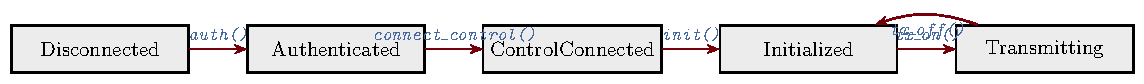
\includegraphics[width=0.85\textwidth]{figures/fig_state_machine.pdf}
\caption{Connection state machine. Each transition corresponds to a method call on \texttt{RadarConnection}.}
\label{fig:state-machine}
\end{figure}

The five states are:

\begin{enumerate}[leftmargin=2em]
\item \textbf{Disconnected} --- initial state. No TCP connections exist.
\item \textbf{Authenticated} --- the 44-byte auth payload has been sent to TCP port 10010 and the radar responded with status byte 0x64. The auth TCP connection is then closed.
\item \textbf{ControlConnected} --- a TCP connection to port 10100 has been established with \texttt{TCP\_NODELAY} enabled, and the \texttt{\$N00,CLIENTCONNECTION} message has been received.
\item \textbf{Initialized} --- the firmware query (\texttt{\$R96}) and all $\sim$184 init register reads have been sent and their responses received.
\item \textbf{Transmitting} --- the TX ON command (\texttt{\$S69,2,...}) has been sent. Echo data is flowing on multicast.
\end{enumerate}

Transitions are enforced by state checks: \texttt{connect\_control()} requires at least \texttt{Authenticated}, \texttt{init()} requires \texttt{ControlConnected}, and \texttt{tx\_on()}/\texttt{tx\_off()} require \texttt{Initialized} or \texttt{Transmitting}. Calling a method in the wrong state returns \texttt{RadarError::InvalidState}.

\subsection{RadarError Enum}
\label{subsec:radar-error}

\begin{table}[H]
\centering
\begin{tabularx}{\textwidth}{l X}
\toprule
\textbf{Variant} & \textbf{Meaning} \\
\midrule
\texttt{AuthFailed(String)} & Auth response was absent or had unexpected status byte \\
\texttt{ConnectionFailed(String)} & TCP connection to radar could not be established \\
\texttt{IoError(std::io::Error)} & Low-level I/O error (read/write failure) \\
\texttt{Timeout} & Operation exceeded its deadline \\
\texttt{InvalidState\{expected, actual\}} & Method called in wrong connection state \\
\texttt{ProtocolError(String)} & Malformed response or unexpected protocol behavior \\
\bottomrule
\end{tabularx}
\caption{\texttt{RadarError} variants.}
\label{tab:radar-error}
\end{table}

\subsection{Timeout Values}
\label{subsec:timeouts}

\begin{table}[H]
\centering
\begin{tabular}{l r l}
\toprule
\textbf{Operation} & \textbf{Timeout} & \textbf{Notes} \\
\midrule
Authentication TCP connect & 5\,s & \texttt{TcpStream::connect\_timeout} \\
Auth response read & 3\,s & Socket read timeout \\
Control channel TCP connect & 5\,s & \texttt{TcpStream::connect\_timeout} \\
Initial message read & 2\,s & Waiting for \texttt{\$N00,CLIENTCONNECTION} \\
Init register responses & 3\,s & Bulk read after sending $\sim$184 queries \\
Command acknowledgment & 3\,s & \texttt{send\_and\_read\_ack} default \\
Subsequent read (within burst) & 200\,ms & Short timeout for trailing messages \\
Keepalive interval & 5\,s & Echo thread sends if elapsed \\
Echo socket read & 500\,ms & UDP receive timeout \\
\bottomrule
\end{tabular}
\caption{Timeout values used throughout the connection lifecycle.}
\label{tab:timeouts}
\end{table}

\subsection{Graceful Degradation}
\label{subsec:graceful-degradation}

The web server starts even if the initial radar connection fails. In \texttt{start\_server()}, if \texttt{connect\_full()} returns an error, the \texttt{connected} flag is set to \texttt{false} and a warning is printed. The HTTP server still binds its port and serves the web interface. All API endpoints that require a radar connection check the \texttt{connected} flag and return an error message directing the user to the \texttt{/reconnect} endpoint.

The \texttt{/reconnect} endpoint creates a fresh \texttt{RadarConnection}, drops the old one, and attempts \texttt{connect\_full()} again. On success, it updates the \texttt{connected} flag and resets \texttt{tx\_active} to false.

\subsection{Keepalive Handling}
\label{subsec:keepalive-handling}

The radar expects periodic keepalive packets on the control channel. If keepalives stop, the radar drops the client connection after approximately 30 seconds.

In web mode, the echo listener thread handles keepalives. Every 5 seconds (checked via \texttt{last\_keepalive.elapsed()}), it acquires the connection mutex via \texttt{try\_lock()} (non-blocking to avoid deadlocking with HTTP handlers), sends the 8-byte binary keepalive packet, and calls \texttt{drain\_control()} to discard any pending control channel data.

In CLI modes, keepalives are sent explicitly by calling \texttt{conn.send\_keepalive()} inside the echo collection loop. The \texttt{drain\_control()} call prevents the TCP receive buffer from filling up with unsolicited telemetry messages.


% ──────────────────────────────────────────────────────────────────────────────
\newpage
\section{Testing \& Validation}
\label{sec:testing}

All tests require a live radar connected to the host. There is no mock or simulation mode.

\subsection{Running Tests}
\label{subsec:running-tests}

\begin{lstlisting}[language=bash]
cd furuno-server
cargo test -- --test-threads=1
\end{lstlisting}

The \texttt{--test-threads=1} flag is required because all tests share a single radar connection, and the radar supports only one authenticated client at a time. Running tests in parallel causes connection conflicts.

\subsection{Test Categories}
\label{subsec:test-categories}

The test suite in \texttt{tests.rs} contains 26 integration tests organized into five categories.

\subsubsection{Connection Tests (6)}
\label{subsubsec:test-connection}

These verify the connection state machine: authentication succeeds with status 0x64, the control channel receives \texttt{\$N00,CLIENTCONNECTION}, initialization completes with firmware data, keepalives are sent and acknowledged, and the echo multicast socket can be created and joined.

\subsubsection{TX Tests (3)}
\label{subsubsec:test-tx}

TX on/off cycling verifies that \texttt{tx\_on()} transitions to the \texttt{Transmitting} state and \texttt{tx\_off()} returns to \texttt{Initialized}. Echo reception verifies that multicast packets arrive after TX ON. Full rotation collection verifies that the rotation wrap detection correctly identifies a complete $360°$ sweep.

\subsubsection{Settings Tests (14)}
\label{subsubsec:test-settings}

Each settings test follows a set-and-read pattern: send a \texttt{\$S} command to change a parameter, then send the corresponding \texttt{\$R} query and verify the response contains the expected value. Parameters tested include range, gain, pulse width, sea clutter, rain clutter, RezBoost, antenna revolution, near/middle/far STC, main bang, interference rejection, bird mode, and Doppler.

\subsubsection{Echo Impact Tests (2)}
\label{subsubsec:test-echo-impact}

These tests verify that parameter changes produce measurable differences in echo data. The gain impact test compares mean echo amplitude at low vs high gain. The range impact test compares sweep parameters (sweep length, spoke count) at short vs long range. These are environment-dependent and may produce SKIP/WARN results if the radar is not receiving returns.

\subsubsection{Render Integration Test (1)}
\label{subsubsec:test-render}

The render integration test exercises the complete pipeline: receive UDP echo packets, decode them into \texttt{Spoke} structs, render via \texttt{render\_ppi()}, encode to PNG via \texttt{encode\_png\_bytes()}, and verify the result is a valid PNG with non-zero size.

\subsection{A/B Command Testing}
\label{subsec:ab-testing}

The \texttt{test-commands} CLI mode (\texttt{testing.rs}) provides a more visual form of testing. For each of 18 parameters, it captures a full rotation PPI image before and after applying a command, then saves both as PNG files. An operator can visually compare the before/after pairs to verify command effects.

Each test follows a setup--before--apply--after--restore sequence. The setup command establishes a known baseline. The ``before'' capture collects one rotation at the baseline. The ``apply'' command changes the parameter. The ``after'' capture collects one rotation with the new setting. The restore command returns to the baseline.

Results are saved to \texttt{test\_output/} with filenames like \texttt{01\_range\_2nm\_BEFORE.png} and \texttt{01\_range\_2nm\_AFTER.png}. A summary table at the end shows ACK status and echo statistics for each test.

\subsection{Validation Suite}
\label{subsec:validation-suite}

The \texttt{validate} CLI mode runs the comprehensive 6-phase test described in \S\ref{subsec:cli-validate}. It produces a timestamped output directory containing CSV files, PNG captures, and a \texttt{report.txt} with PASS/FAIL/SKIP counts and detailed per-test output. The validation suite tests 14 parameters in A/B/A fashion (3 checks each = 42 assertions), plus connection, TX, and echo impact tests, for a total of approximately 47 individual assertions.


% ══════════════════════════════════════════════════════════════════════════════
%
%   PART III — ECHO DATA PIPELINE
%
% ══════════════════════════════════════════════════════════════════════════════

\newpage
\part{Echo Data Pipeline}
\label{part:echo}


% ──────────────────────────────────────────────────────────────────────────────
\section{Echo Data Format}
\label{sec:echo-data-format}

\subsection{Packet Structure}
\label{subsec:echo-packet-structure}

% TODO: Figure — echo UDP packet layout

\subsection{Header Field Breakdown}
\label{subsec:echo-header}

% TODO: 16-byte header field-by-field

\subsection{Echo Metadata Extraction}
\label{subsec:echo-metadata}

% TODO: sweep_count, sweep_len, encoding extraction formulas

\subsection{Spoke Sub-Header}
\label{subsec:spoke-subheader}

% TODO: 4-byte layout per spoke: 2 bytes azimuth (u16 LE) + 2 bytes heading (u16 LE)

\subsection{Multi-Spoke Packing}
\label{subsec:multi-spoke}

% TODO: How multiple spokes are packed sequentially; sweep_count tells how many

\subsection{Azimuth and Heading}
\label{subsec:azimuth-heading}

% TODO: 8192 ticks per full rotation, compass bearing convention

\subsection{Typical Packet Characteristics}
\label{subsec:echo-packet-characteristics}

% TODO: Sizes and rates observed at different range settings


% ──────────────────────────────────────────────────────────────────────────────
\newpage
\section{Echo Encoding Types}
\label{sec:echo-encoding}

% TODO: Overview — 4 encoding schemes, selected by header field

\subsection{Encoding 0: Raw Uncompressed}
\label{subsec:encoding-0}

% TODO: Direct byte storage + 4-byte alignment padding rule

\subsection{Encoding 1: RLE with Repeat Marker}
\label{subsec:encoding-1}

% TODO: LSB=0 literal, LSB=1 repeat; worked byte-level example

\subsection{Encoding 2: Delta RLE with Previous Spoke Reference}
\label{subsec:encoding-2}

% TODO: Like Encoding 1 but repeats copy from previous spoke; worked example

\subsection{Encoding 3: 2-Bit RLE with Dual Reference}
\label{subsec:encoding-3}

% TODO: 2-bit control; worked example showing both repeat and copy modes

\subsection{Encoding Selection}
\label{subsec:encoding-selection}

% TODO: Which encodings are observed at which ranges/conditions

\subsection{Display Value Conversion}
\label{subsec:display-conversion}

% TODO: display = wire >> 2

\subsection{Rotation Detection}
\label{subsec:rotation-detection}

% TODO: Echo listener detects wrap-around when azimuth drops by >1000 ticks


% ──────────────────────────────────────────────────────────────────────────────
\newpage
\section{Doppler Processing}
\label{sec:doppler}

\subsection{Status Field Encoding}
\label{subsec:doppler-status}

% TODO: Bit layout table

\subsection{Echo Byte Encoding}
\label{subsec:doppler-echo-byte}

% TODO: Normal (full 8-bit) vs Doppler (bit 7 = D flag, bits 6:0 = 7-bit intensity)

\subsection{Downstream Usage}
\label{subsec:doppler-downstream}

% TODO: How the D bit is used after decoding

\subsection{Practical Notes}
\label{subsec:doppler-practical}

% TODO: What "moving target" looks like in real data, reliability, range limitations


% ──────────────────────────────────────────────────────────────────────────────
\newpage
\section{Dual-Pulse Interleaving}
\label{sec:dual-pulse}

\subsection{Pulse Types}
\label{subsec:pulse-types}

% TODO: Long (17 discrete levels, full quantization table) vs short (130-240 continuous)

\subsection{Range Dependence}
\label{subsec:pulse-range-dependence}

% TODO: Ratio table by range setting

\subsection{Rez Boost Effect}
\label{subsec:pulse-rez-boost}

% TODO: How rez boost shifts the long/short ratio and short-pulse resolution

\subsection{Spoke Handling}
\label{subsec:pulse-spoke-handling}

% TODO: How the code treats long vs short pulse spokes


% ══════════════════════════════════════════════════════════════════════════════
%
%   PART IV — NETWORK & WIRE PROTOCOL
%
% ══════════════════════════════════════════════════════════════════════════════

\newpage
\part{Network \& Wire Protocol}
\label{part:protocol}


% ──────────────────────────────────────────────────────────────────────────────
\section{Network Architecture}
\label{sec:network-architecture}

\subsection{Topology}
\label{subsec:network-topology}

% TODO: Figure — network topology

\subsection{Port Map}
\label{subsec:port-map}

% TODO: Port table

\subsection{Auto-Discovery and Network Configuration}
\label{subsec:auto-discovery}

% TODO: Three-stage fallback logic

\subsubsection{Platform-Specific IP Alias}
\label{subsubsec:ip-alias}

% TODO: Linux: ip addr add, macOS: ifconfig alias, Windows: placeholder only


% ──────────────────────────────────────────────────────────────────────────────
\newpage
\section{Control Protocol}
\label{sec:control-protocol}

\subsection{Message Format}
\label{subsec:message-format}

% TODO: $S (set), $R (read), $N (notify) prefixes, comma-separated params, \r\n terminated

\subsection{Binary Keepalive}
\label{subsec:keepalive}

% TODO: 8-byte packet, sent every 5s + figure

\subsection{Binary vs ASCII Disambiguation}
\label{subsec:binary-ascii}

% TODO: Exact 8-byte match for keepalive, not just "check first byte"

\subsection{Response Types}
\label{subsec:response-types}

% TODO: RadarResponse enum — ClientConnection, Keepalive, RegisterValue, Unknown

\subsection{Response Parsing Pipeline}
\label{subsec:response-parsing}

% TODO: read_responses(), partial line buffering, parse_response_line()

\subsection{Command Acknowledgment}
\label{subsec:command-ack}

% TODO: send_and_read_ack() — deadline-based waiting

\subsection{Control Channel Drain}
\label{subsec:drain-control}

% TODO: drain_control() — flush pending data without parsing

\subsection{Initialization Sequence}
\label{subsec:init-sequence}

% TODO: 6 phases + figure

\subsubsection{Phase 1: Discovery}
\label{subsubsec:init-discovery}

% TODO: UDP beacon on port 10010

\subsubsection{Phase 2: Authentication}
\label{subsubsec:init-auth}

% TODO: TCP 10010, 44-byte payload with copyright string, expect byte[9]=0x64

\subsubsection{Phase 3: Control Channel}
\label{subsubsec:init-control}

% TODO: TCP 10100 with TCP_NODELAY, expect $N00,CLIENTCONNECTION

\subsubsection{Phase 4: Firmware Query}
\label{subsubsec:init-firmware}

% TODO: $R96,,,,,,,\r\n, response stored in self.firmware

\subsubsection{Phase 5: Register Dump}
\label{subsubsec:init-registers}

% TODO: ~184 $R commands covering registers 0x61-0xFF

\subsubsection{Phase 6: Steady State}
\label{subsubsec:init-steady}

% TODO: Keepalives every 5-10s, heading reports at ~1Hz


% ──────────────────────────────────────────────────────────────────────────────
\newpage
\section{Command Reference}
\label{sec:command-reference}

% TODO: Complete command reference with corrected IDs verified against protocol.rs

\subsection{TX State (\texttt{\$S69})}
\label{subsec:cmd-tx}

% TODO: state: 1=standby, 2=transmit; always accompanied by STC resets

\subsection{Range (\texttt{\$S62})}
\label{subsec:cmd-range}

% TODO: wire_index mapping table (18 entries, 1/16 NM to 48 NM)

\subsection{Gain (\texttt{\$S63})}
\label{subsec:cmd-gain}

% TODO: auto/manual mode, value 0-255, maxGain=80 hardcoded as 4th param

\subsection{Sea Clutter (\texttt{\$S64})}
\label{subsec:cmd-sea}

% TODO: Basic (status, value) and full variant (sea_mode: 0=Advanced, 1=Coastal)

\subsection{Rain Clutter (\texttt{\$S65})}
\label{subsec:cmd-rain}

% TODO: Basic and full variant (ftc_mode: 0=OFF, 1=FTC-1, 2=FTC-2; rain_mode)

\subsection{Pulse Width (\texttt{\$S68})}
\label{subsec:cmd-pulse}

% TODO: pulse value 0-5 (S1/S2/M1/M2/M3/L) + range_index as second param

\subsection{STC Near (\texttt{\$S85})}
\label{subsec:cmd-stc-near}

% TODO: value 0-4

\subsection{STC Middle (\texttt{\$S86})}
\label{subsec:cmd-stc-middle}

% TODO: value 0-3

\subsection{STC Far (\texttt{\$S87})}
\label{subsec:cmd-stc-far}

% TODO: value 0-2

\subsection{Main Bang Suppression (\texttt{\$S83})}
\label{subsec:cmd-main-bang}

% TODO: value 0-255

\subsection{Antenna Height (\texttt{\$S84})}
\label{subsec:cmd-antenna-height}

% TODO: meters above sea level

\subsection{Antenna Revolution (\texttt{\$S89})}
\label{subsec:cmd-antenna-revolution}

% TODO: speed (0=LO, 1=HI, 2=AUTO) + hi_rpm flag

\subsection{Interference Rejection (\texttt{\$S67}, param[2]=2)}
\label{subsec:cmd-ir}

% TODO: value: 0=off, 2=on

\subsection{Noise Reduction (\texttt{\$S67}, param[2]=3)}
\label{subsec:cmd-noise}

% TODO: value: 0=off, 1=on

\subsection{Rez Boost (\texttt{\$SEE})}
\label{subsec:cmd-rezboost}

% TODO: level 0-3

\subsection{Bird Mode (\texttt{\$SED})}
\label{subsec:cmd-bird}

% TODO: level 0-3

\subsection{Doppler / Target Analyzer (\texttt{\$SEF})}
\label{subsec:cmd-doppler}

% TODO: mode: 0=off, 1=target, 2=rain

\subsection{No-Transmit Sectors (\texttt{\$S77})}
\label{subsec:cmd-no-transmit}

% TODO: 2 sectors, angles in degrees with 360-degree wrapping

\subsection{Query Commands}
\label{subsec:cmd-queries}

% TODO: Full table of all $R query commands with IDs and expected response format


% ──────────────────────────────────────────────────────────────────────────────
\newpage
\section{Periodic Telemetry}
\label{sec:telemetry}

\subsection{Telemetry Message Table}
\label{subsec:telemetry-table}

% TODO: $NAF,256; $NF5; $NE0; $N83,100,1; $N68; $N00,CLIENTCONNECTION; keepalive

\subsection{Telemetry Processing}
\label{subsec:telemetry-processing}

% TODO: How read_responses() categorizes incoming data via RadarResponse enum

\subsection{Parsed vs Discarded Data}
\label{subsec:telemetry-parsed}

% TODO: Register values logged, keepalives acknowledged, unknown lines stored


% ──────────────────────────────────────────────────────────────────────────────
\newpage
\section{Proprietary Library Reference}
\label{sec:proprietary-lib}

\subsection{Module Breakdown}
\label{subsec:lib-modules}

% TODO: libNAVNETDLL.so module breakdown table

\subsection{Shared Command IDs}
\label{subsec:lib-shared-ids}

% TODO: $R67 controls multiple features via sub-parameter


\end{document}
